%   Filename    : chapter_4.tex 
\chapter{Results and Discussions}

\section{System Display}

\begin{figure}[!htbp]
	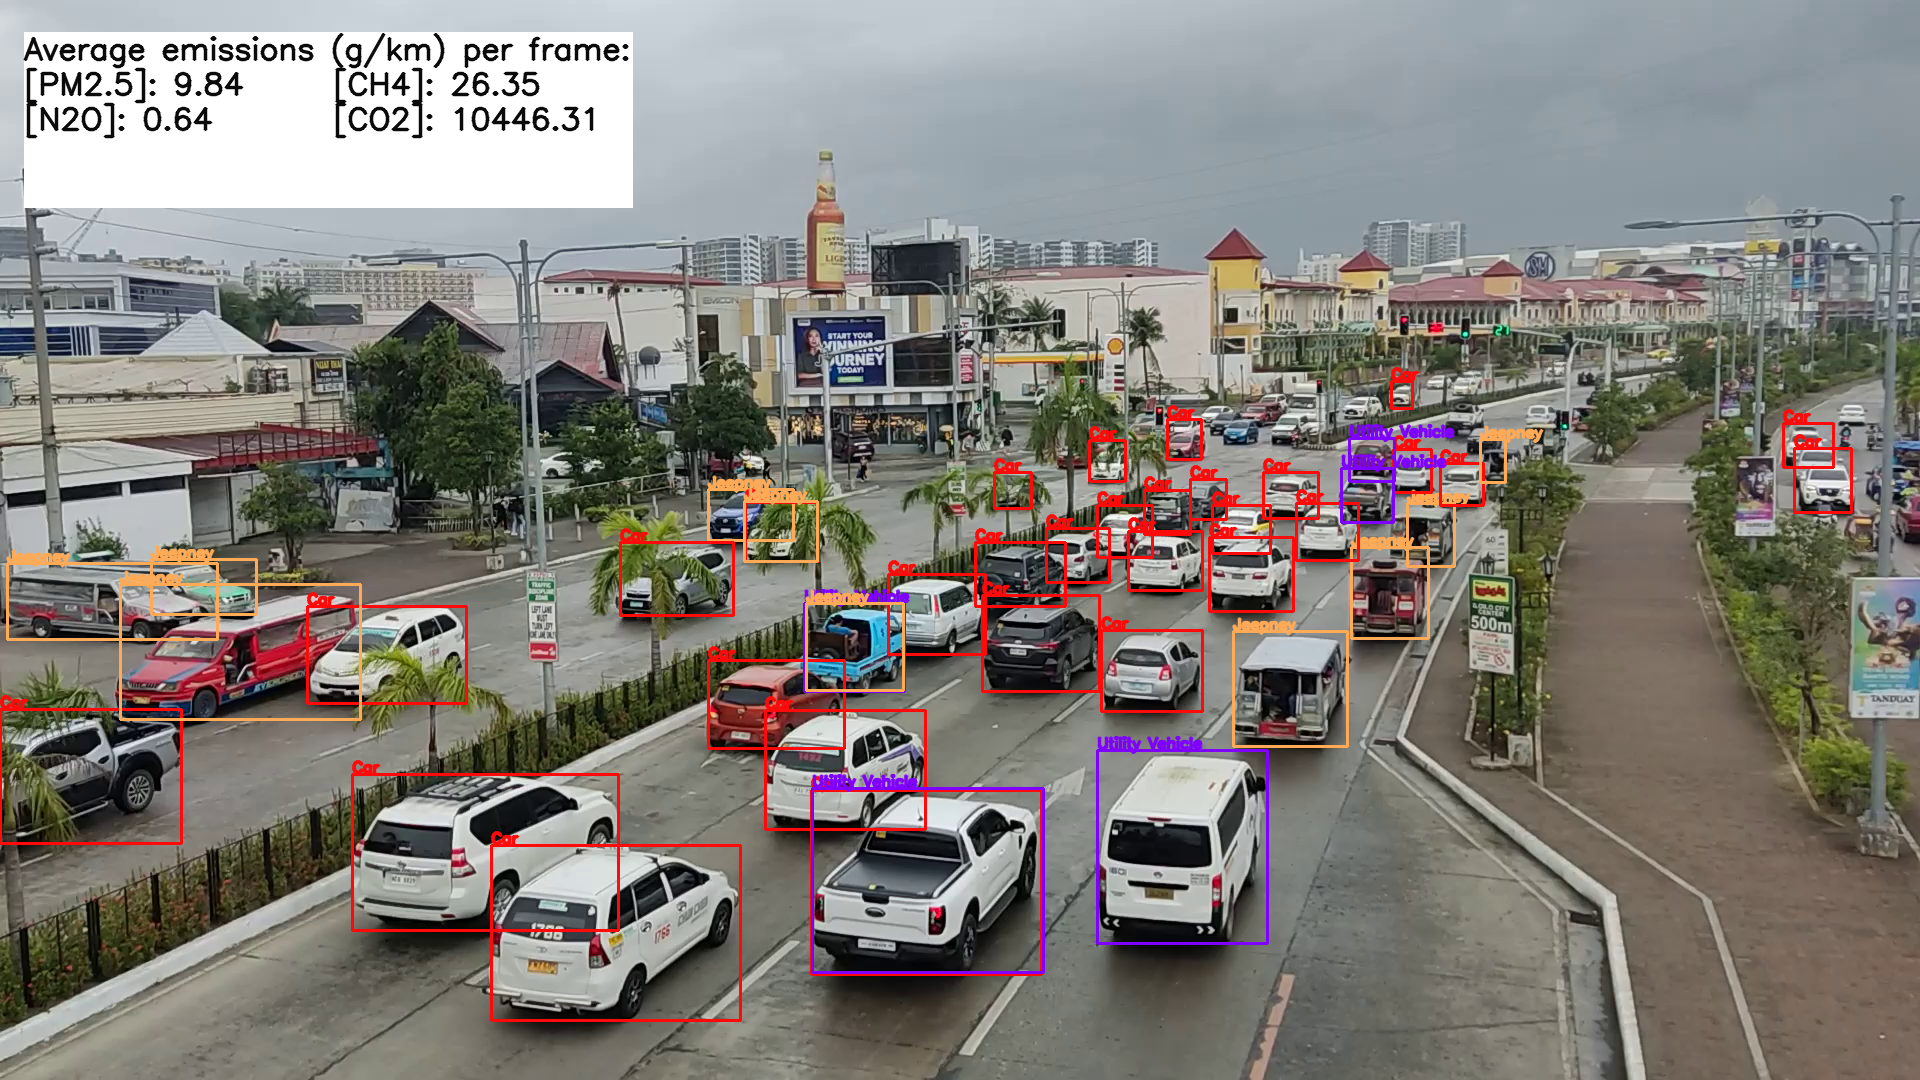
\includegraphics[width=\linewidth,scale=0.8]{display_sample.png}
	\caption{Ha.Zee system display showing the vehicles being detected and the pollutants estimated}
	\label{fig:display}
\end{figure}
\FloatBarrier

Figure \ref{fig:display} shows the Ha.Zee system and what it displays. The bounding boxes are placed over the vehicles they detect, along with the name and colors assigned per vehicle type. The average emissions per frame is displayed on the upper left of the screen, showing the estimated emissions of the pollutants: $PM_{2.5}$, \ch{CH4}, \ch{N2O}, and \ch{CO2}. The rectangular space where the text is displayed is colored white to provide readability of the information.



\section{Training Results}

\subsection{Loss Values and Metric Progression}
After training the dataset, the YOLOv5 algorithm provided statistics to show how the model performs and progresses after a certain number of epochs, which in this study, 100 epochs were used.



Figure \ref{fig:graph} shows the statistics of how the data set performed during training. The loss values used in the graph were box loss, objectness loss, and classification loss. These loss values represent the performance of the model during training concerning the ground truth \cite{
Hui_2022}. Box loss refers to the errors in the location and size of the predicted boundaries, objectness or confidence loss measures the probability that an object exists in the region of interest, and classification loss measures how effective the model is in predicting the correct class. The graph shows that as the training progresses the loss values followed a downward progression which meant that the model is making fewer errors as training continues for both the train and validation sets.

\begin{figure}[!htbp]
	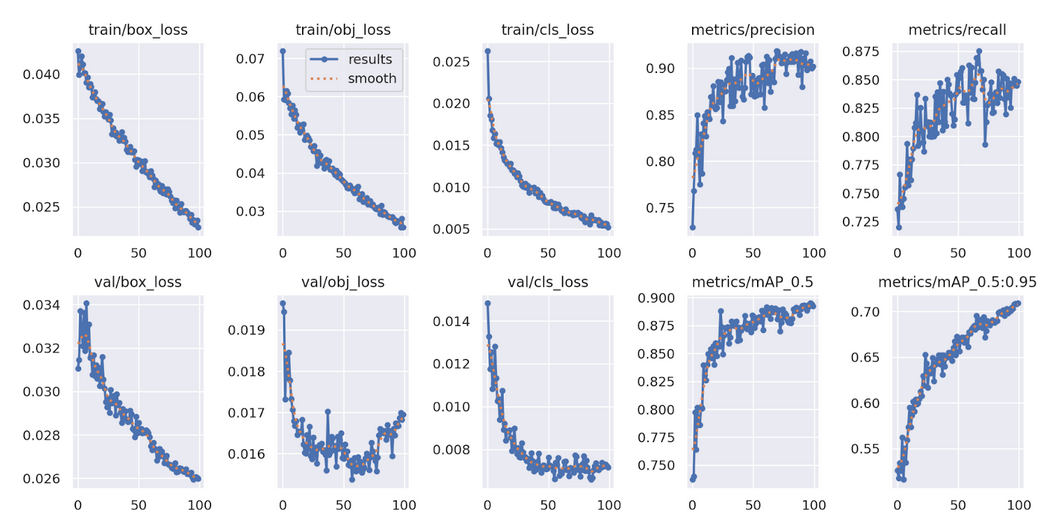
\includegraphics[width=\linewidth,scale=0.8]{statistics.png}
	\caption{Graphs depicting the loss values (object, box, classification) and metric progressions (precision, recall, and mean average precision) during training with 100 epochs}
	\label{fig:graph}
\end{figure}
\FloatBarrier

For the metric values there is precision, mean average precision, and recall. Recall is a metric that measures the portion of the true values that are predicted true while precision measures the portion of the predicted values that are true \cite{D_Powers}. Mean average precision was calculated by averaging the precision of each class and then averaging all the precision of every class \cite{Shah_2022}. In the graph, the metrics show an upward, although not linear, progression along 100 epochs, which means that the model is improving continuously for training and validation. 
 

\subsection{Confusion Matrix/F-1 Score Calculation}
After training the model, a confusion matrix was provided (figure \ref{fig:con_mat}) which depicts the normalized count of predicted versus true values of the six (6) classes and the background in the model, and is useful for getting the metrics necessary to measure the performance of the model.
The normalization of the confusion matrix was obtained by dividing each of the row's elements to the sum of the entire row. The normalized elements all add up to 1.0. This allows the matrix to be read in percentages.

The diagonal boxes (which are dark blue in figure \ref{fig:con_mat})indicate the true positives, wherein the predicted vehicle during training is actually the proper vehicle type. The true positives of every vehicle all have a good score, with tricycles having the highest value of 0.90 or 90\% accurately detected as tricycles. 

The columns, excluding the diagonal elements (dark blue) of true positives, indicate the false negatives. These are instances where the vehicle was detected as another type (i.e. 1\% of cars were detected as either a jeepney, motorcycle, or utility vehicle).

The "background" class was included for the instance where the detected object is anything but vehicle. The background row signifies the percentages of the vehicles not being detected. Meanwhile, the background column signifies the instances where a vehicle was detected but in actuality, the detected object is part of the background or is not a vehicle. The background does not have true positive as it is not part of the training process.


 The confusion matrix was made using the validation set of the training data with a confidence of 0.25 based on the source code of YOLOv5. This might cause discrepancies when running the model with real-world data as the confidence value might vary. 


\begin{figure}[!htbp]
	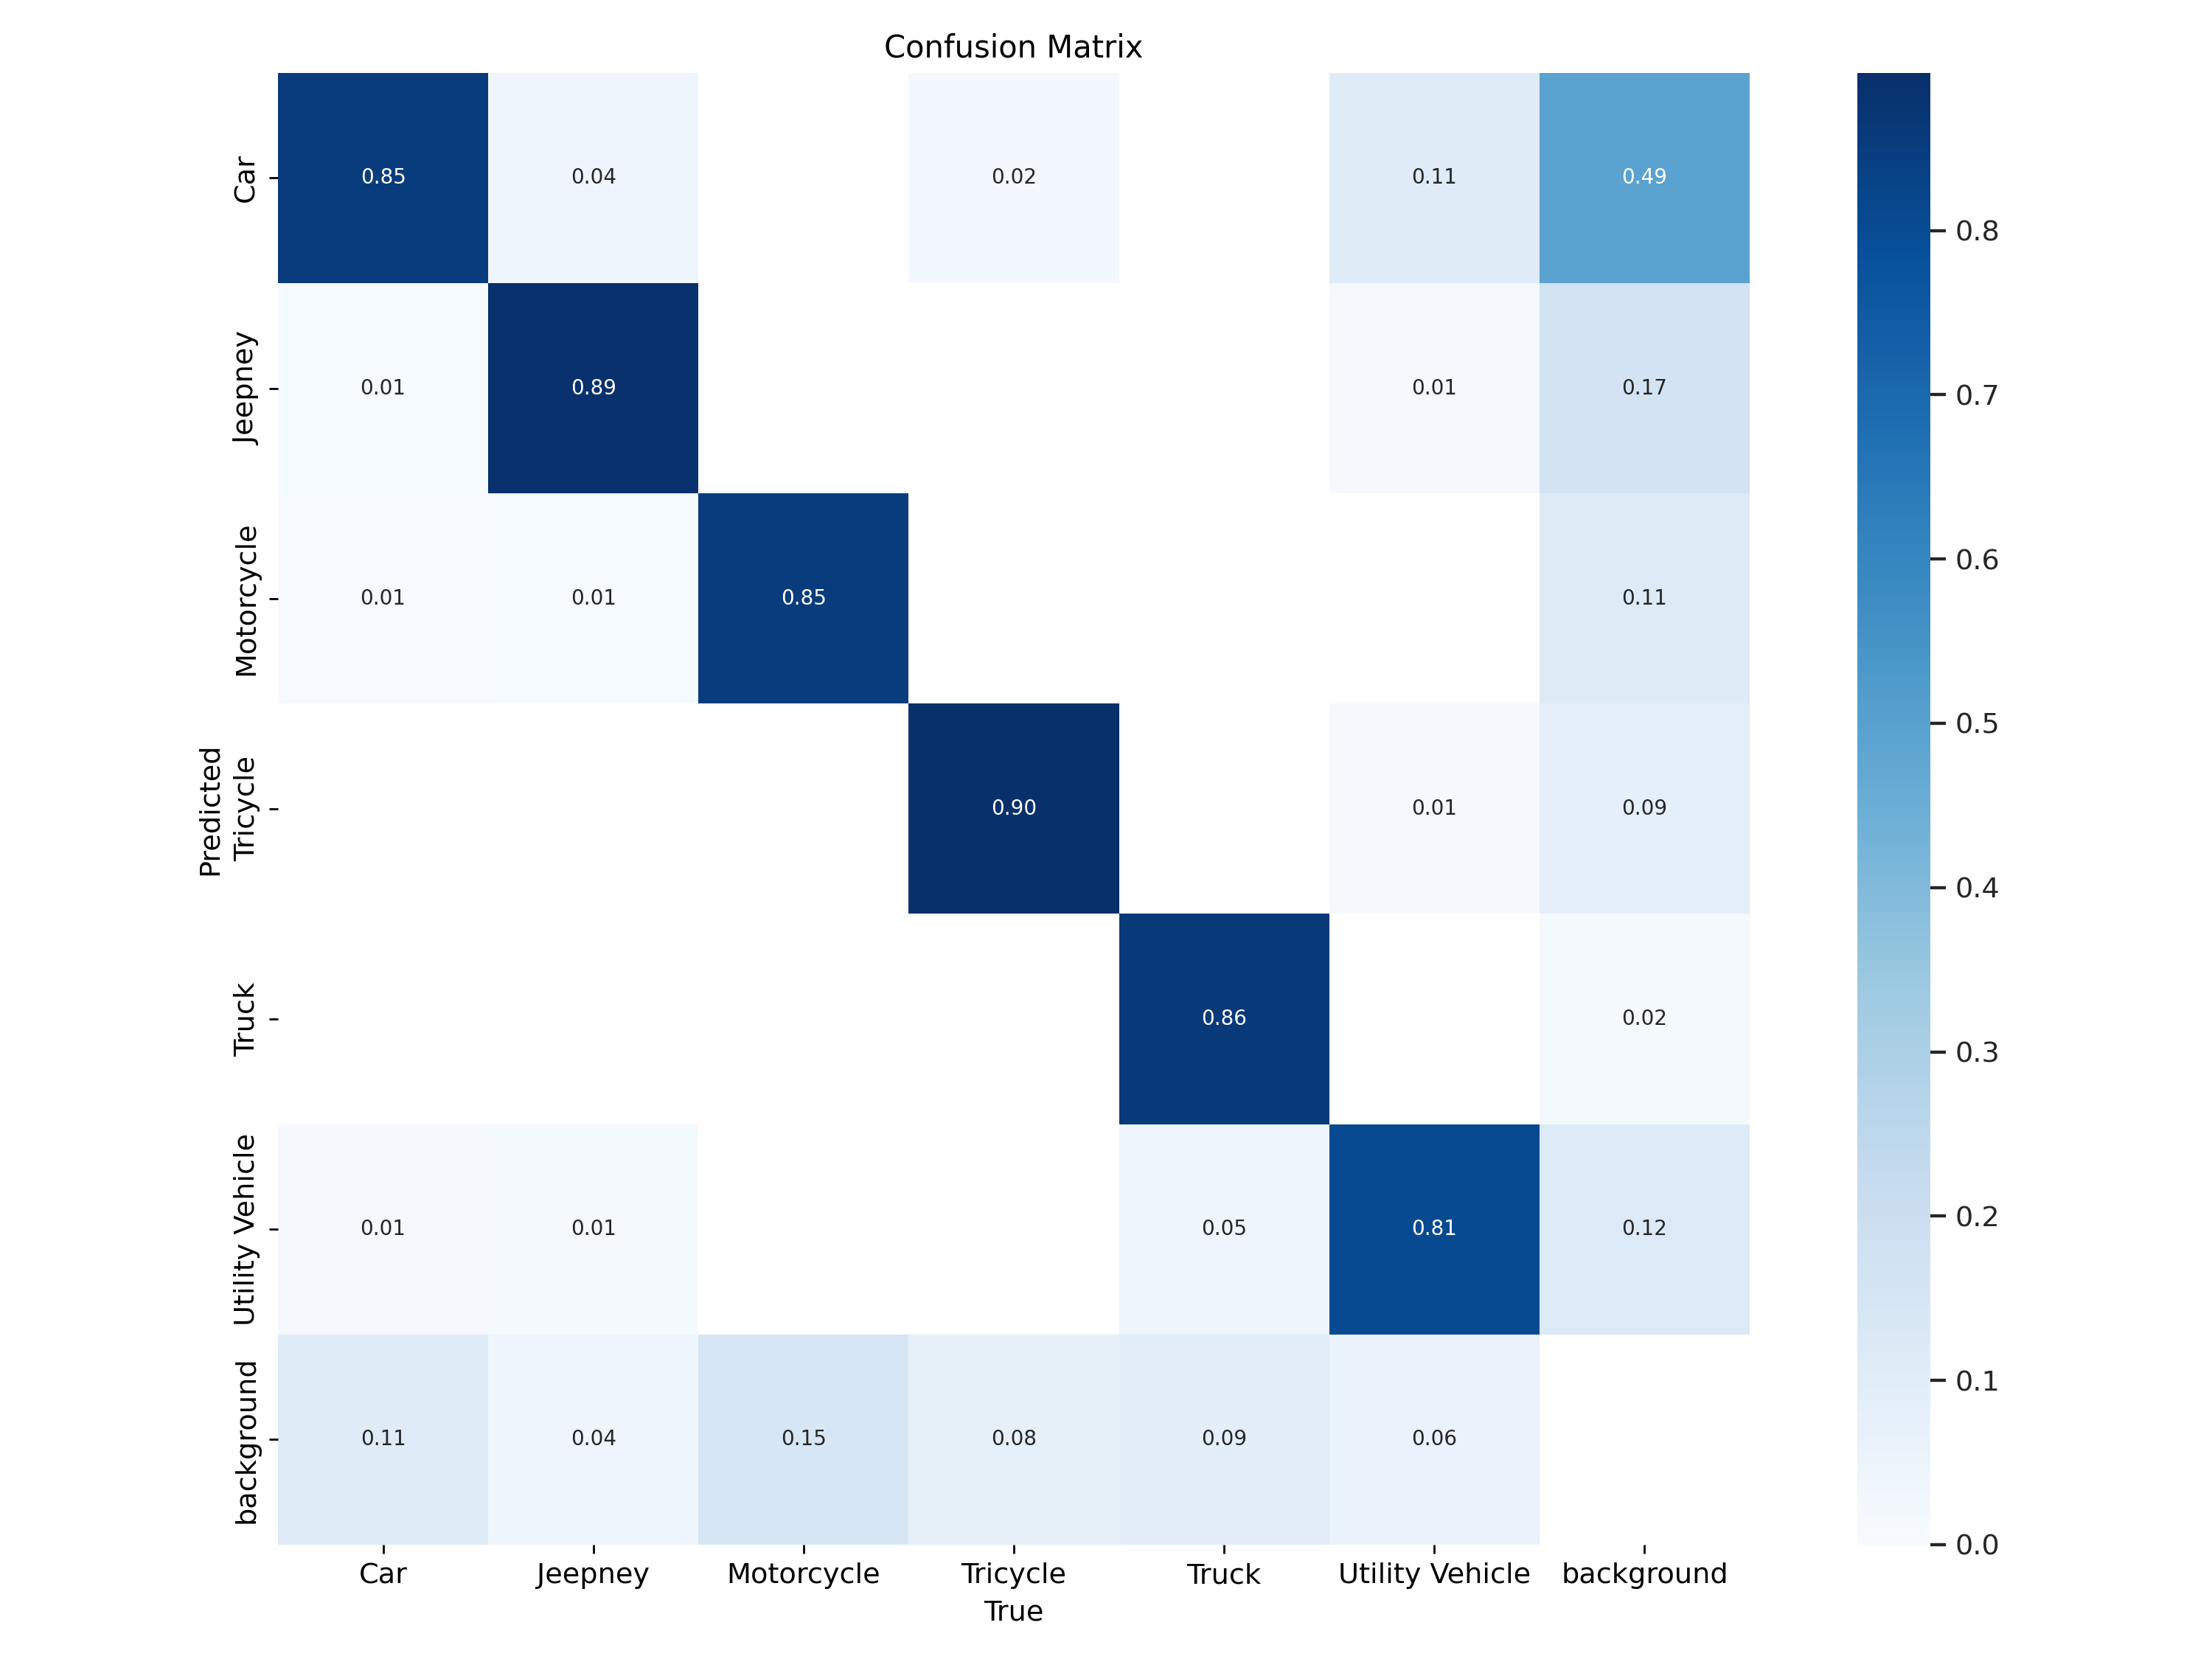
\includegraphics[width=\linewidth,scale=0.8]{confusion_matrix.png}
	\caption{Confusion matrix of the training; Values are normalized}
	\label{fig:con_mat}
\end{figure}
\FloatBarrier

For this system, the F1-score metric was used because there was a class imbalance due to the limitations of the locations where the data was taken as shown in Figure \ref{fig:class_bal}. F1-score is a better metric to use compared to accuracy when there is a class imbalance because it measures using the number and type of errors, unlike accuracy which only calculated the number of correct predictions \cite{Korstanje_2021}. Furthermore, the researchers decided that accuracy is not an ideal metric to represent what the model should be predicting, because as a multi-class object detection model that relies on the exact number of vehicles to calculate for emission, it is important to take into account not only the number of correct predictions but also the type of errors, which is what the F1-score metric provides. However, for comparison, the macro averages of the accuracy metric and F1-score metric will be calculated.  




To get the F1-score for multi-class classification must be calculated first with the following formulas which were taken from the Towards Data Science article \cite{Korstanje_2021} and from Powers \citeyear{D_Powers}:

\begin{equation} \label{eq:accuracy}
	{\text{Accuracy}}= \frac{\text{Correct Predictions}}{\text{Total Predictions}} 
\end{equation}


\begin{equation} \label{eq:[precision]}
{\text{Precision}}= \frac{\text{class TP}}{\text{class TP}+\text{class FP}} 
\end{equation}

\begin{equation} \label{eq:recall}
{\text{Recall}}= \frac{\text{class TP}}{\text{class TP}+\text{class FN}} 
\end{equation}


\begin{equation} \label{eq:F1}
{\text{F1}}= 2 * \frac{\text{Precision}*\text{Recall}}{\text{Precision}+\text{Recall}} 
\end{equation}


For calculating the precision, we can get the values available in the confusion matrix in Figure 4.1. In the following example, the precision for the “Car” class is calculated using the formula from equation \ref{eq:accuracy}:

\[{\text{Precision\textsubscript{Car}}}= \frac{0.85}{0.85+(0.04+0+0.02+0+0.11+0.49)} \]

\[{\text{Precision\textsubscript{Car}}}= \frac{0.85}{1.51} \]

\[{\text{Precision\textsubscript{Car}}}= 0.5629139073 \]

The value 0.85 was taken from the cell of the predicted and true value for the “Car” class which means that it is a true positive because the predicted objects were the true objects. The false positives from the matrix are the other classes that are predicted as the “Cars” class in the confusion matrix. Applying equation \ref{eq:recall} for the recall value of the “Car” class:


\[{\text{Recall\textsubscript{Car}}}= \frac{0.85}{0.85+(0.01+0.01+0+0+0.01+0.11)} \]

\[{\text{Recall\textsubscript{Car}}}= \frac{0.85}{0.99} \]

\[{\text{Recall\textsubscript{Car}}}= 0.8585858586 \]

Similar for the calculation of precision, we get 0.85 as true positive from the confusion matrix. In this case, however, the formula uses false negatives which are classes from the confusion matrix that detected a car for objects that are not cars. As stated by equation \ref{eq:F1}, the F1-score can be calculated using both precision and recall. Applying the equation to the "Car" class:

\[{\text{F1}\textsubscript{Car}}= 2 * \frac{0.5629139073*0.8585858586}{0.5629139073+0.8585858586} \]

\[{\text{F1}\textsubscript{Car}}= 2 * \frac{0.4833099204}{1.421499766} \]

\[{\text{F1}\textsubscript{Car}}= 2 * 0.34 \]

\[{\text{F1}\textsubscript{Car}}= 0.68 \]

Lastly, to calculate for accuracy the number of true predictions (true positive and true negatives) was divided by all the values in the confusion matrix. Applying equation \ref{eq:accuracy} for the accuracy value of the “Car” class:

\[{\text{Accuracy}\textsubscript{Car}}= \frac{0.85 + 5.33}{6.98} \]

\[{\text{Accuracy}\textsubscript{Car}}=  \frac{6.18}{6.98} \]


\[{\text{Accuracy}\textsubscript{Car}}= 0.8853868195 \]


With this methods, the performance metrics of each class was calculated and the results are shown in Table \ref{tab:perf_mat}. 


\begin{table}[ht]   %t means place on top, replace with b if you want to place at the bottom
	\centering
	\caption{Table of performance metrics of each class} \vspace{0.25em}
	\begin{tabular}{c|c|c|c|c} \hline
		\centering \textbf{Class} & \textbf{Precision} & \textbf{Recall} & \textbf{F1-Score} & \textbf{Accuracy}\\ \hline
		Car & 0.5629139073 & 0.8585858586  & 0.68 & 0.8853868195 \\ \hline
		Jeepney & 0.8240740741 & 0.898989899  & 0.8599033816 & 0.9584527221\\ \hline
		Motorcycle& 0.8673469388  & 0.85   & 0.8585858586 & 0.9598853868 \\ \hline
		Tricycle   & 0.9   & 0.9 & 0.9 & 0.9713467049\\ \hline
		Truck & 0.9772727273 & 0.86 & 0.914893617 & 0.9770773639 \\ \hline
		Utility & 0.81 & 0.81 & 0.81 & 0.9455587393\\ \hline
		
	\end{tabular}
	\label{tab:perf_mat}
\end{table}


Table \ref{tab:perf_mat} showed the Precision value calculated from each class. In the table the class with the lowest precision is the “Car” class which is also the class with the most samples, this is due to the “Car” class being over-represented in the dataset therefore making the system overfit for that particular class, meaning it might detect a car even though it should be a different object \cite{Raj_2019}. On the contrary, the “Truck” class had the highest precision value of approximately 0.9773, which meant that every time the model detects a truck there is a high chance that the model has predicted true \cite{D_Powers}, even though the “Truck” class was underrepresented in the dataset. This might be because the trucks are sparse in the testing dataset thus making errors rare. Meanwhile, for recall, the “Tricycle” class had the highest value, (0.9) which meant that the model has a high chance of detecting true tricycles in a frame \cite{D_Powers}. Finally, all classes not including the “Car” class had an F1-score of at least 80\%. The “Car” class has an F1-score of 68\%, the lowest of all classes in this model, which was contributed by its low precision value.The accuracy of the model closely follows the ranking of the F1-scores, the only difference is that the ranks of the “Jeepney” and “Motorcycle” classes swapped places for the accuracy metric, also the accuracy of each class was at least 88\%. The lower accuracy observed for the "Car" class can be attributed to overfitting on the dataset. Consequently, the limited presence of "Truck" class made it less prone to misclassifications or mistakes, thus yielding a higher accuracy for this particular class compared to others.


To find the overall F1-score of the model the macro average of the F1-scores was used. Macro averages were used instead of micro and weighted averages because macro averages put equal importance on all the classes in the model whereas weighted averages are ideal for datasets with classes having different degrees of importance and micro averages are ideal for datasets with a balanced distribution of classes \cite{Leung_2022}. The Macro averages can be calculated by finding the average of the F1-score and accuracy metric from each class \cite{Leung_2022}. To find the macro average of the F1-score and accuracy the average of their respective column were calculated from Figure 4.3.

Equation:
\begin{equation}
	{\text{metric}}= \frac{\text{sum of all values of the metric}}{\text{number of classes}} 
\end{equation}

For F1-score:

\[{\text{F1}}= \frac{0.68 + 0.8599033816 + 0.8585858586 + 0.9 + 0.914893617 + 0.81}{6} \]

\[{\text{F1}}=  \frac{5.023382857}{6} \]


\[{\text{F1}}= 0.8372304762 \]

For Accuracy:


\[{\text{Accuracy}}= \frac{0.89 + 0.96 + 0.96 + 0.97 + 0.98 + 0.95}{6} \]

\[{\text{Accuracy}}=  \frac{5.70}{6} \]


\[{\text{Accuracy}}= 0.95 \]

The model had an accuracy of approximately 95\% not taking into account the errors it made. However, if the errors were considered the model only has an accuracy of approximately 84\% which is lower but is more ideal for the imbalance distribution of classes in the dataset. Nonetheless, the model was accurate enough to be used for object detection.




\section{Object Detection}

The weights obtained through training were used in pre-recorded videos to determine if the weights were trained successfully and to see how they perform in actual video footage. The following locations were chosen by the researchers to be used for the study: Valeria St. , De Leon St., Diversion Road, Lacson St., Roxas Ave. Valeria St. , De Leon St., Diversion Road are located in Iloilo City, Iloilo; Lacson St. is located at Bacolod City, Negros Occidental; and Roxas Ave. is located at Roxas City, Capiz.  The locations were chosen for their variety in vehicle congestion and vehicle type (i.e. Diversion Road with a higher vehicle count; Roxas with more tricycles).  These recordings were then processed using the custom vehicle detection Python program. The “processing” includes detecting the vehicles; drawing bounding boxes; and calculating and displaying the approximation of the emission of that area. 

Using the trained model,  the following are the results showing the Ha.Zee system detecting vehicles and their respective types, along with the vehicle $PM_{2.5}$ emission tracker displayed on the upper left portion of the frame. The $PM_{2.5}$ value here means the weight of particulate matter of at most 2.5 micrometers in diameter in kilograms for every kilometer. The higher the value for $PM_{2.5}$ the greater the health risk, but the interpretation of the value on the particulate matter and its consequences falls outside the scope of this study.  To validate the detection model of the system, the researchers compared the ground truth of the total vehicles in the frame via manual counting to the detected vehicles. The information on the system’s detected vehicles stored in the CSV file was utilized in this comparison. This section focused on comparing the number of vehicles the system could detect to the actual vehicle count and does not account for the accuracy of identifying the proper vehicle type.

\subsubsection{Valeria St. (MaryMart, Iloilo City)}


\begin{figure}[!htbp]
	\begin{subfigure}{.5\textwidth}
		\centering
		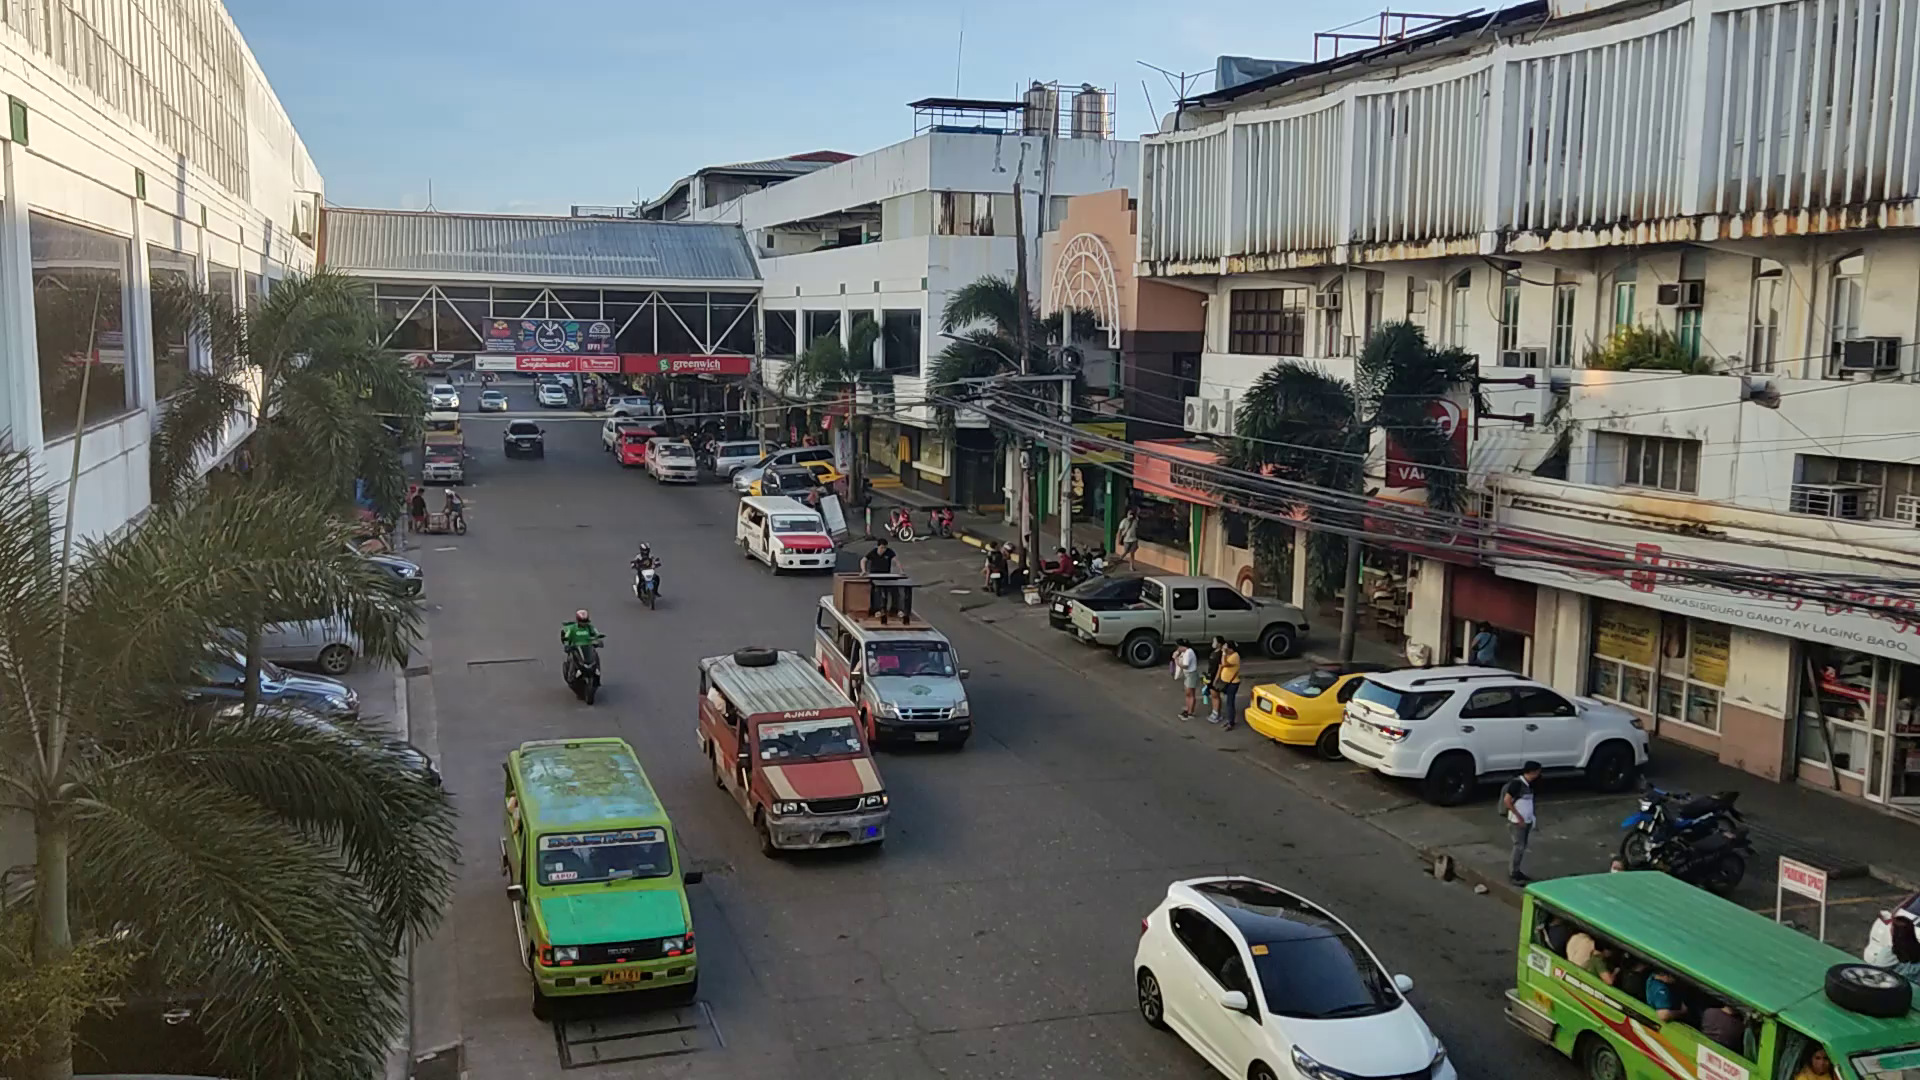
\includegraphics[width=.8\linewidth]{bounding_pics/marymart_unbounded.png}
		\caption{Manual Count: 27 Vehicles}
		
	\end{subfigure}%
	\begin{subfigure}{.5\textwidth}
		\centering
		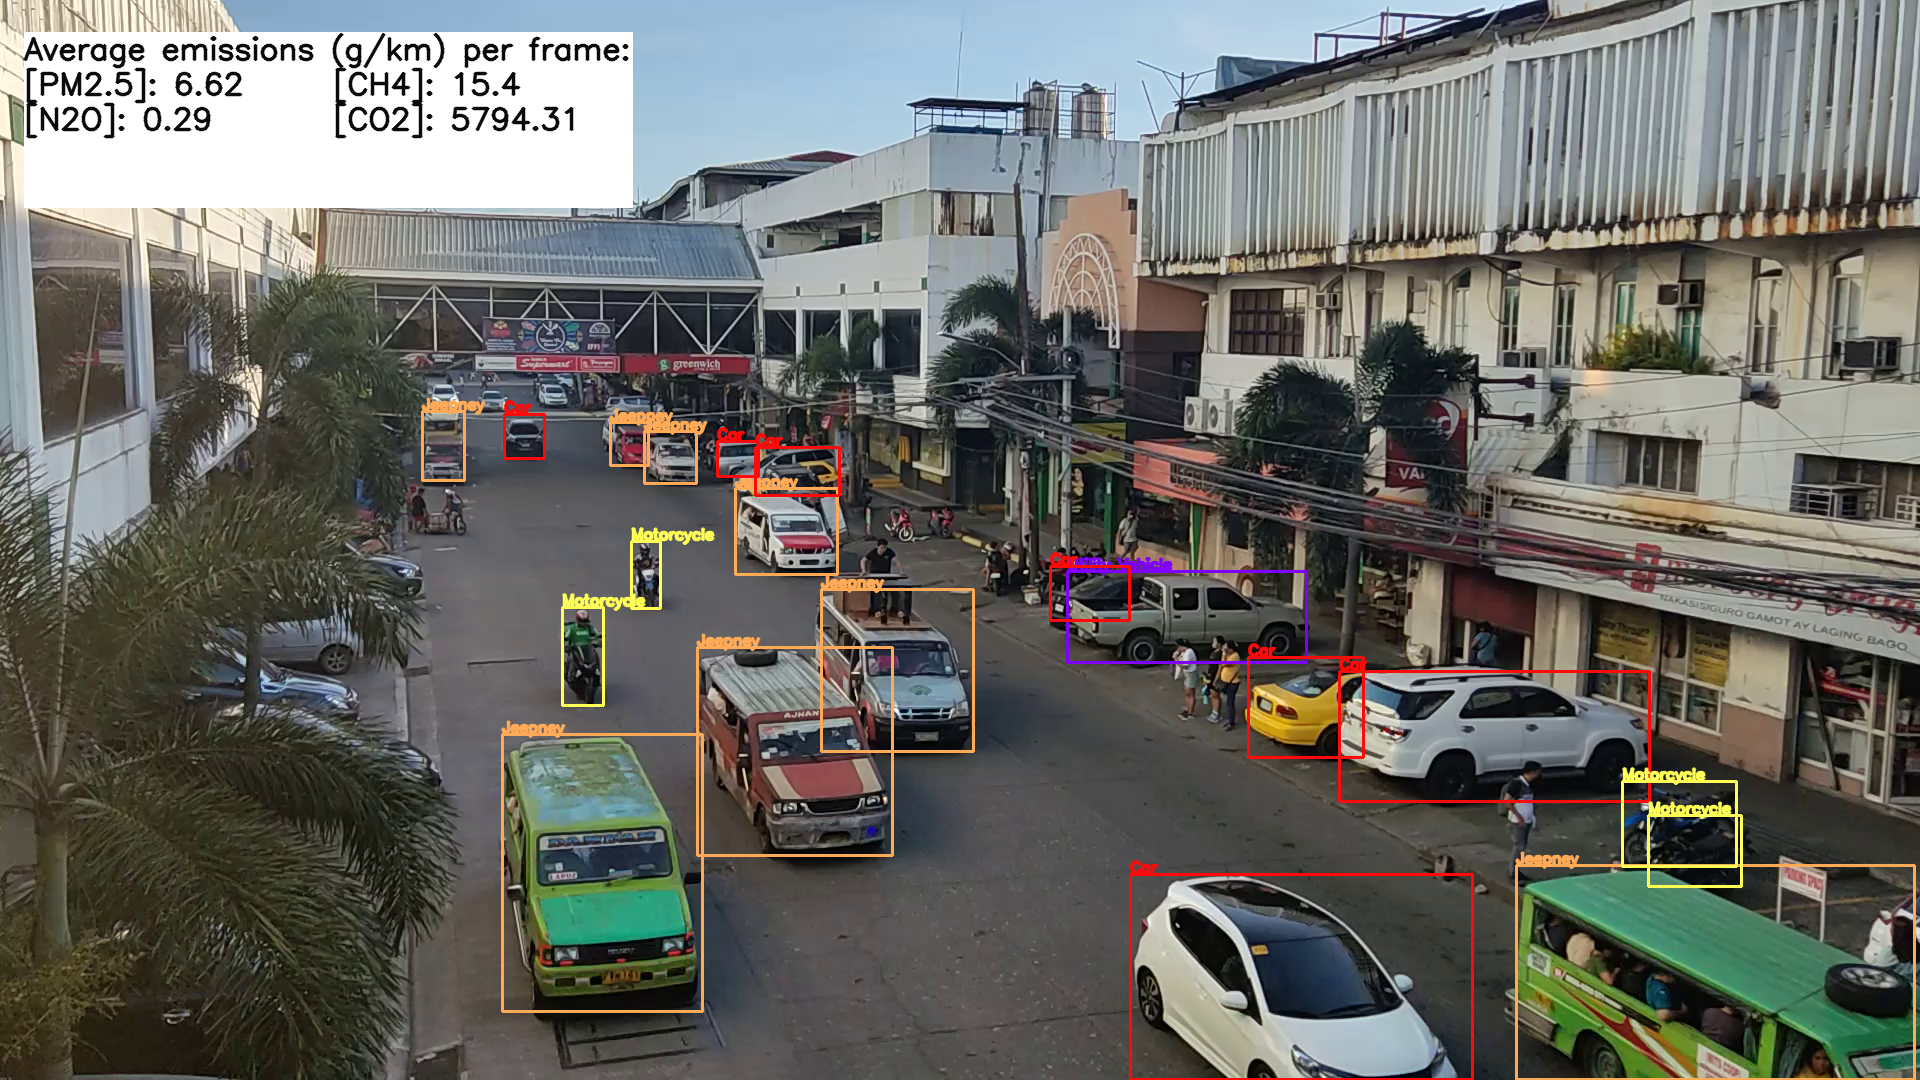
\includegraphics[width=.8\linewidth]{bounding_pics/marymart_bounded.png}
		\caption{Ha.Zee Count: 17 vehicles}
	\end{subfigure}
	\caption{Valeria St. Traffic Video Footage; Date Taken: 2-25-23, 5:01 PM}
	\label{fig:valeria}
\end{figure}
\FloatBarrier

Using the frames from Figure \ref{fig:valeria} to represent the video footage from Valeria St., Iloilo City Proper; the researchers manually counted 27 total vehicles. The most common vehicle in this frame is the car, with a count of 12. After using the trained model, the system returned a count of 17 vehicles. In this instance, the most common vehicle type detected was the jeepney, with a count of 8. The road being a route for jeepneys could have influenced their frequency in appearance.

Table \ref{tab:valeria_st} shows the average of vehicles present over the course of the video duration. The average of vehicles appearing in the video is obtained through the sum of the average of a vehicle type’s appearance per second. The same process was applied to the vehicles detected by the system. The ratio between the two counts is then calculated. Of the total average of manually-counted vehicles, only 64.98\% were detected by the system. 



\begin{table}[ht]   %t means place on top, replace with b if you want to place at the bottom
	\centering
	\caption{Ratio of Manual vs. Detected average vehicles counted  (Valeria St.)} \vspace{0.25em}
	\begin{tabular}{c|c|c} \hline
		\centering \textbf {Vehicle type} & \textbf{Manual Count Avg.} & \textbf{Ha.Zee Count Avg.} \\ \hline
		Car & 11.72 & 4.55   \\ 
		Jeepney & 9.72 & 8.18  	\\ 
		Motorcycle& 4.55  & 3.55   \\ 
		Tricycle   & 0  & 0.09  \\ 
		UV & 3 & 1.18  \\ 
		Truck & 0 & 0 \\ \hline
		
		\textbf{Total Average} &27 & 9.145\\ \hline
		\textbf{Ratio/Percentage} & \multicolumn{2}{c}{0.6498}  \\ \hline
		
	\end{tabular}
	\label{tab:valeria_st}
\end{table}

\newpage
\subsubsection{De Leon St.  (Robinsons Place, Iloilo City)
}


\begin{figure}[!htbp]
	\begin{subfigure}{.5\textwidth}
		\centering
		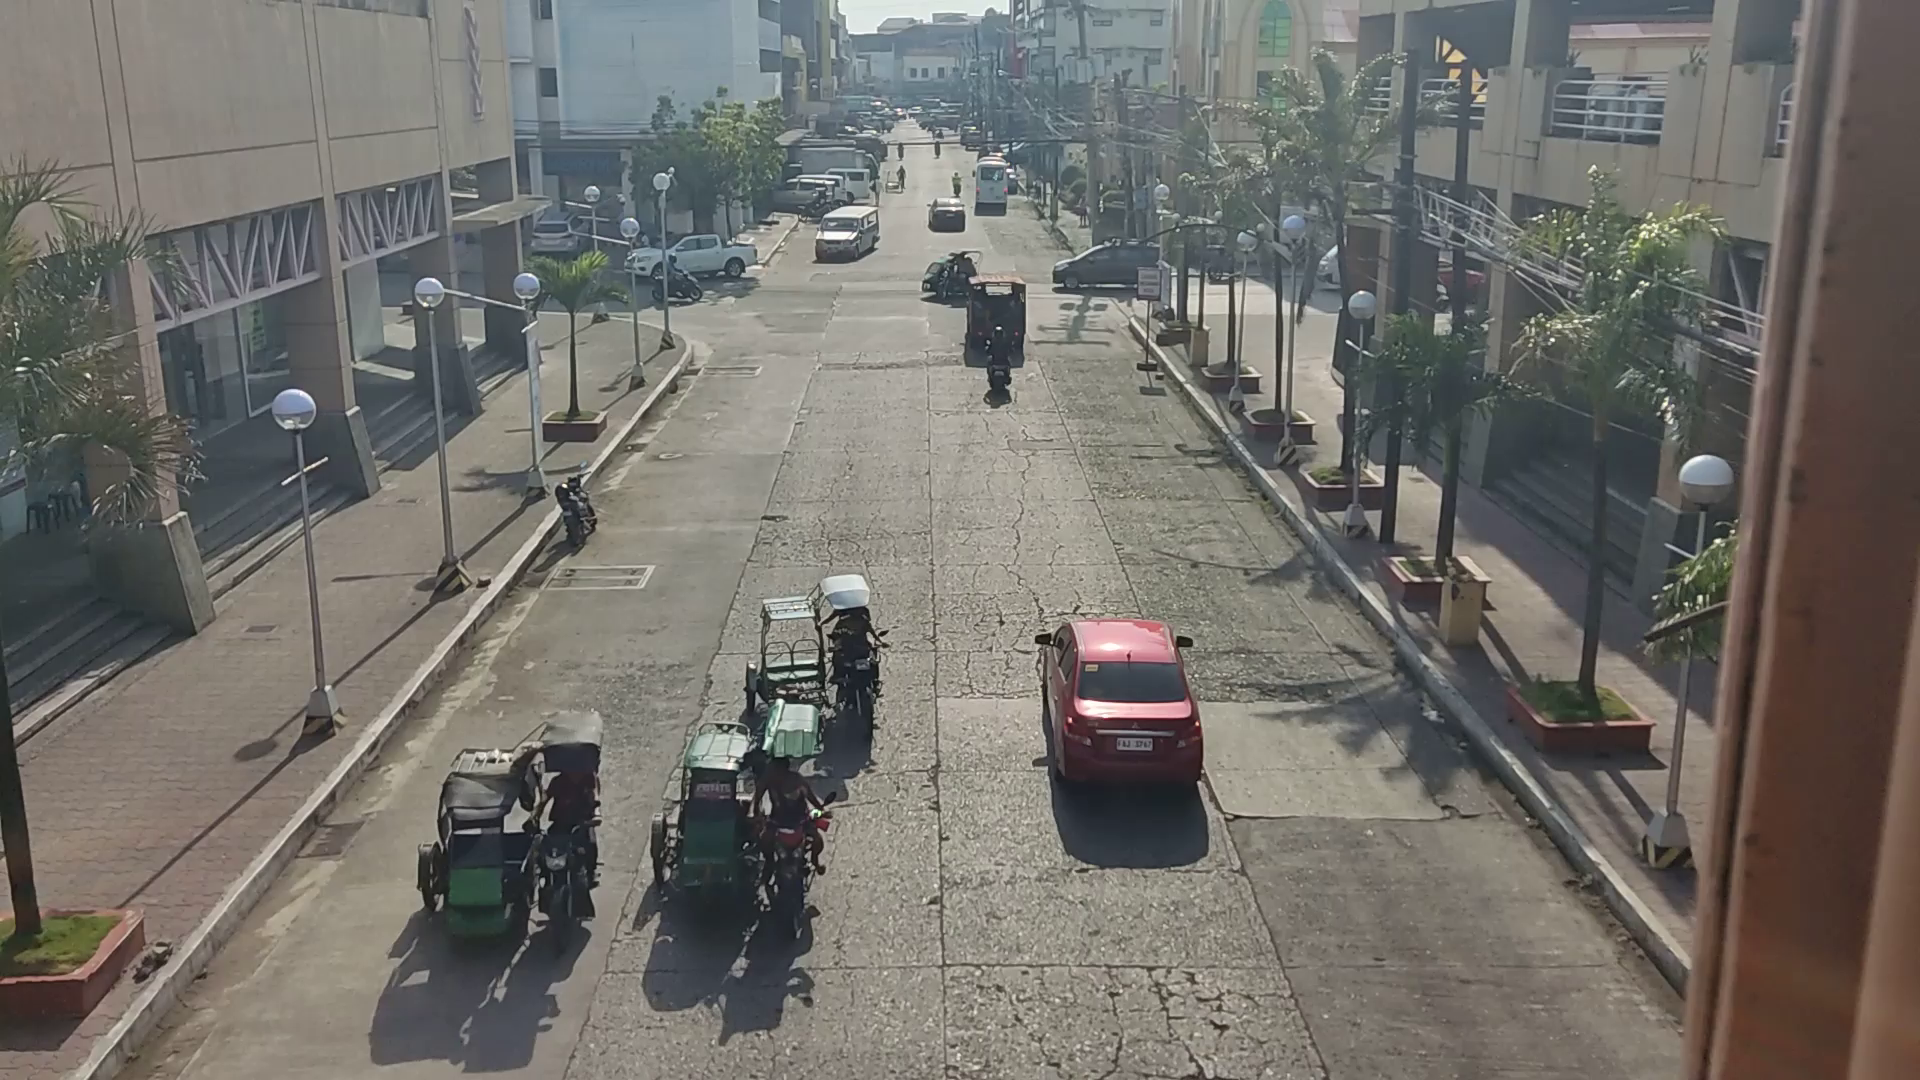
\includegraphics[width=.8\linewidth]{bounding_pics/rob_unbound.png}
		\caption{Manual Count: 15 Vehicles}
		
	\end{subfigure}%
	\begin{subfigure}{.5\textwidth}
		\centering
		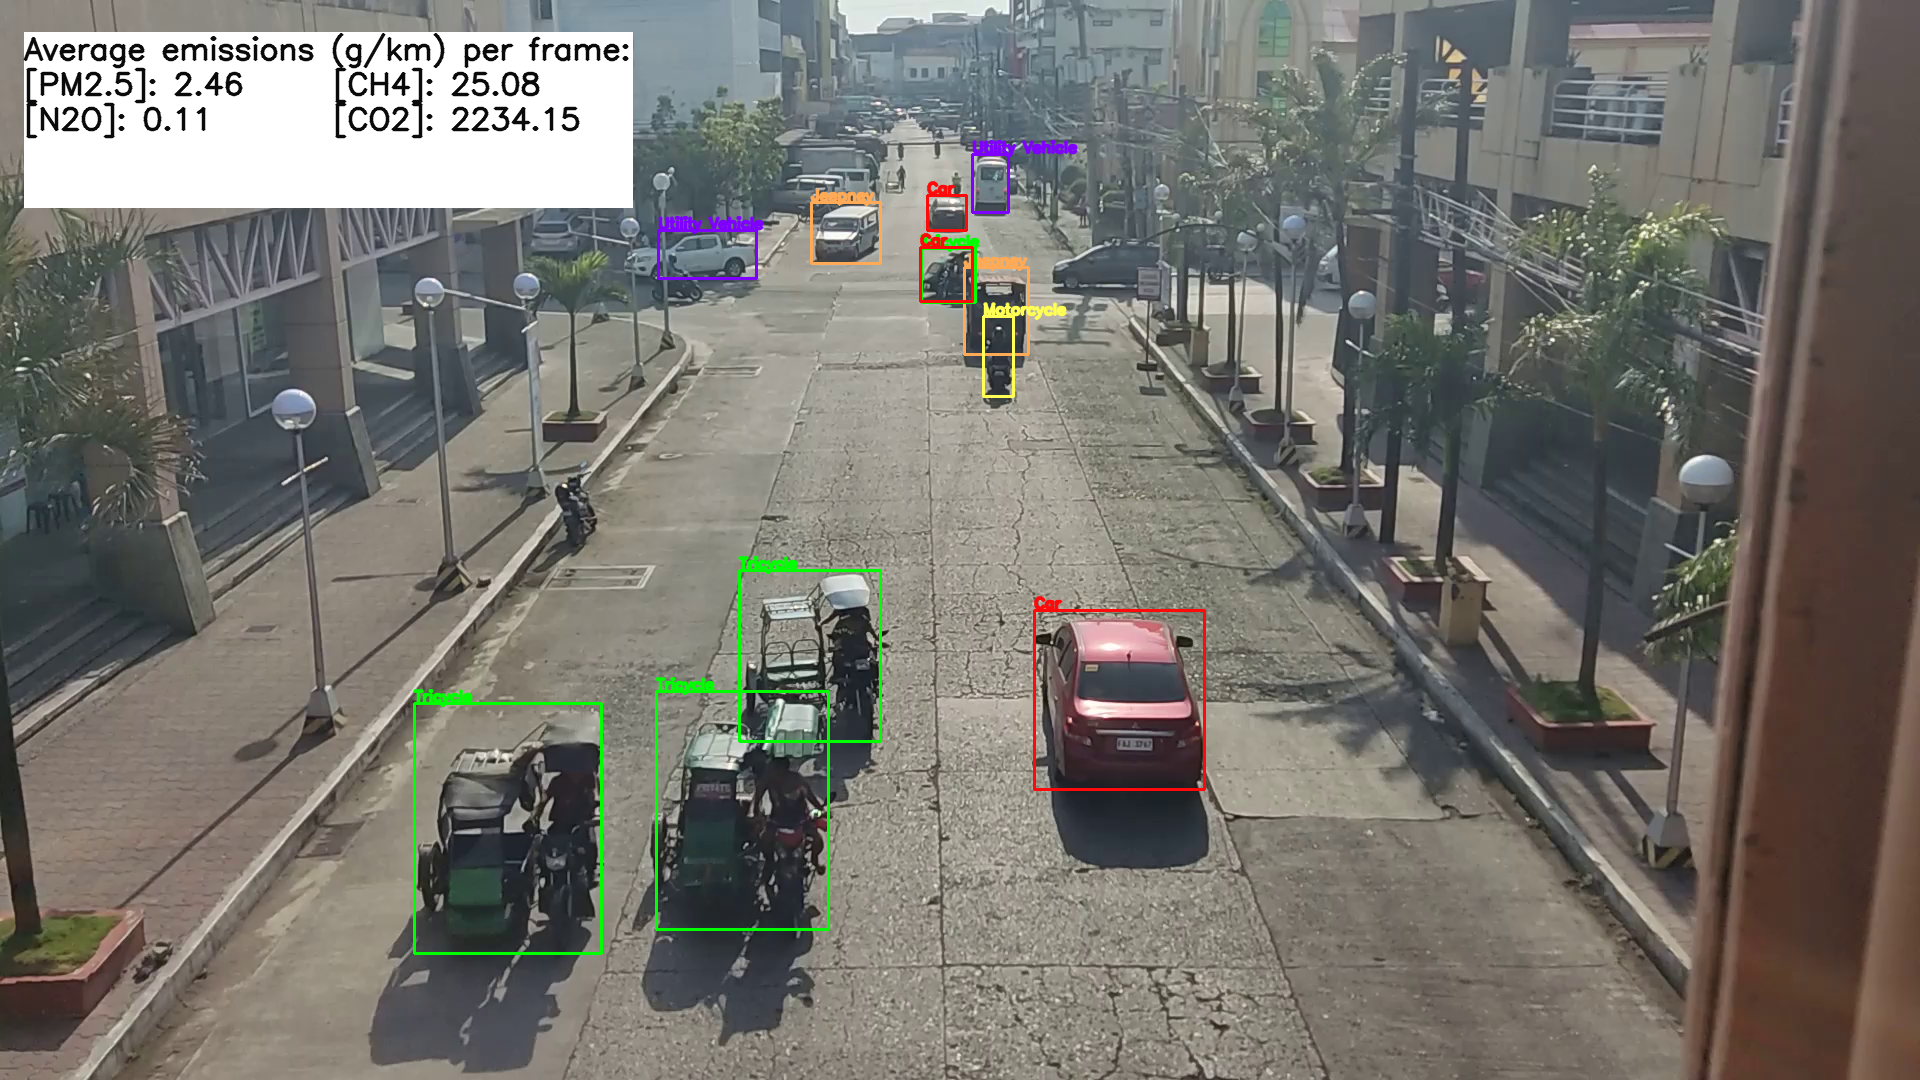
\includegraphics[width=.8\linewidth]{bounding_pics/rob_bound.png}
		\caption{Ha.Zee Count: 10 vehicles}
	\end{subfigure}
	\caption{De Leon St. Traffic Video Footage; Date Taken: 4-5-23, 8:04 AM}
	\label{fig:de_leon}
\end{figure}
\FloatBarrier

Using the frames from Figure \ref{fig:de_leon} to represent the video footage from De Leon St., Iloilo City; the researchers manually counted 15 total vehicles. The most common vehicles in this frame are motorcycles and tricycles, both with a count of 4. After using the trained model, the system returned a count of 10 vehicles. In this instance, the most common vehicle type detected was the jeepneys and tricycles, with a count of 3. It is noted that 2 of the detected jeepneys are false positives.

Table \ref{tab:de_leon} applies the same calculation processes as the previous location. Of the total average of manually-counted vehicles, only 73.28\% were detected by the system. 



\begin{table}[ht]   %t means place on top, replace with b if you want to place at the bottom
	\centering
	\caption{Ratio of Manual vs. Detected average vehicles counted  (De Leon St.)} \vspace{0.25em}
	\begin{tabular}{c|c|c} \hline
		\centering \textbf {Vehicle type} & \textbf{Manual Count Avg.} & \textbf{Ha.Zee Count Avg.}\\ \hline
		Car & 2.63 & 2    \\ 
		Jeepney & 2 & 1.72  	\\ 
		Motorcycle& 3.55  & 1.36  \\ 
		Tricycle   & 3.45  & 3.27  \\ 
		UV & 1.63 & 1.36  \\ 
		Truck & 0 & 0 \\ \hline
		
		\textbf{Total Average} &13.27 & 9.72   \\ \hline
		
		\textbf{Ratio/Percentage} & \multicolumn{2}{c}{0.7328}  \\ \hline
		
	\end{tabular}
	\label{tab:de_leon}
\end{table}

\subsubsection{Diversion Road (Jaro, Iloilo City)
}


\begin{figure}[!htbp]
	\begin{subfigure}{.5\textwidth}
		\centering
		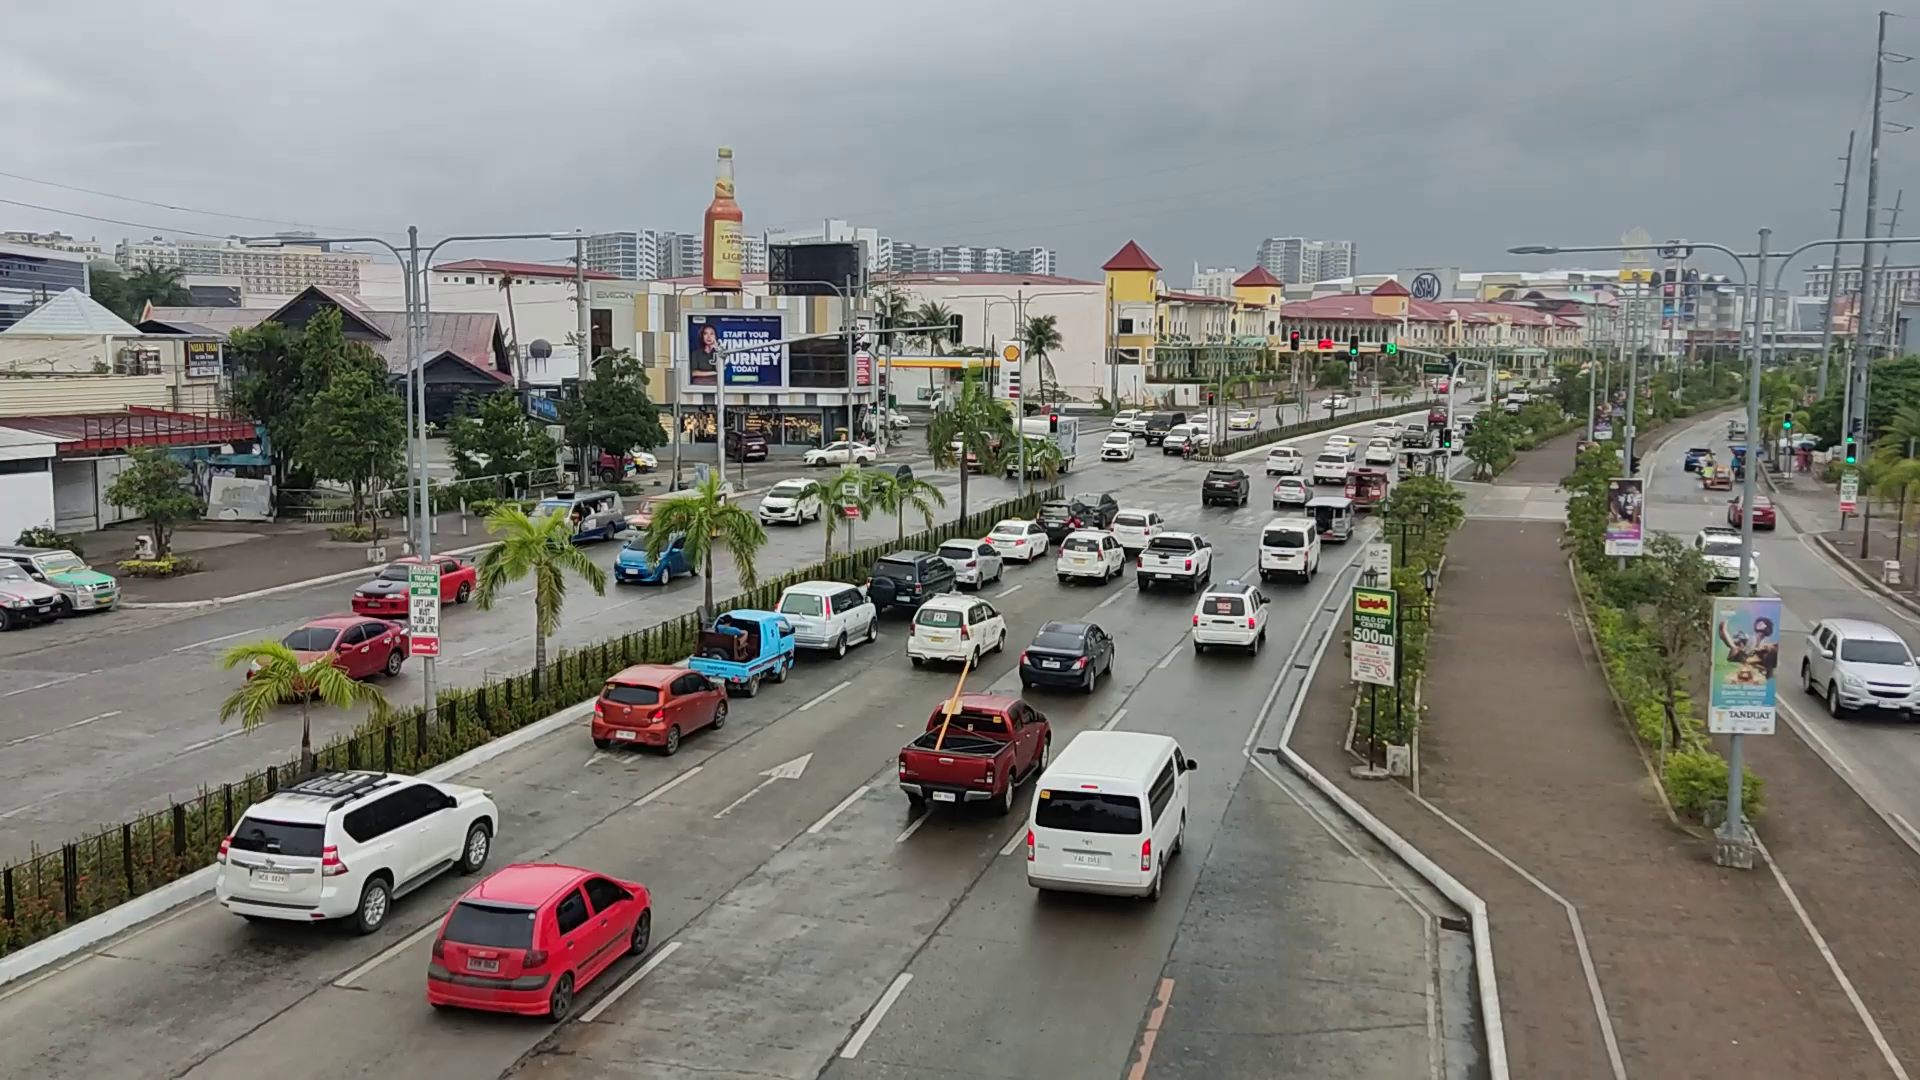
\includegraphics[width=.8\linewidth]{bounding_pics/diversion_unbounded.png}
		\caption{Manual Count: 60 Vehicles}
		
	\end{subfigure}%
	\begin{subfigure}{.5\textwidth}
		\centering
		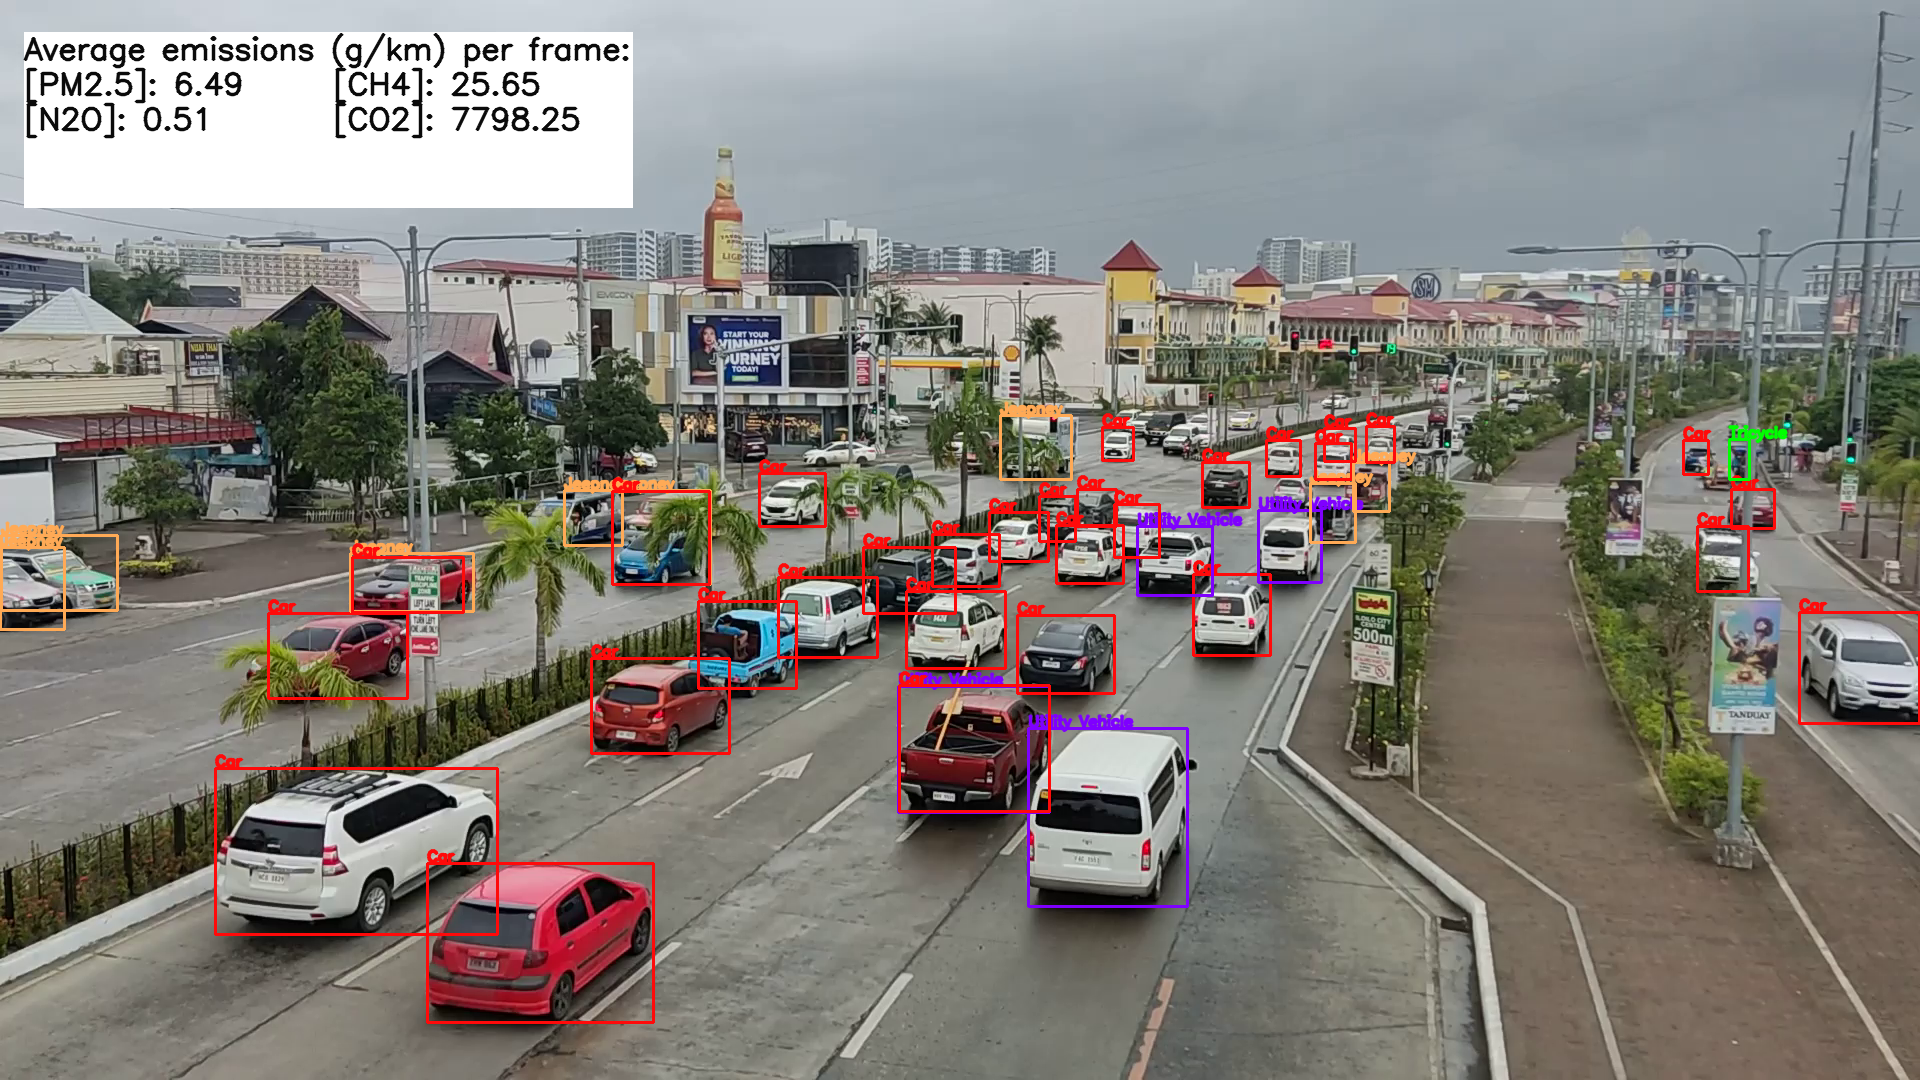
\includegraphics[width=.8\linewidth]{bounding_pics/diversion_bounded.png}
		\caption{Ha.Zee Count: 42 vehicles}
	\end{subfigure}
	\caption{Diversion Road Traffic Video Footage; Date Taken: 2-19-23, 2:13 AM}
	\label{fig:diversion}
\end{figure}
\FloatBarrier

Using the frames from Figure \ref{fig:diversion} to represent the video footage from Diversion Road, Iloilo City; the researchers manually counted 60 total vehicles. The most common vehicle in this frame is the car, with a count of 46. After using the trained model, the system returned a count of 42 vehicles. In this instance, the most common vehicle type detected was also the car, with a count of 27. Cars are a big majority of this video footage, yet have a big gap in the system’s detection.

Table \ref{tab:diversion_rd} applies the same calculation processes as the previous location. Of the total average of manually-counted vehicles, only 71.60\% were detected by the system. 




\begin{table}[ht]   %t means place on top, replace with b if you want to place at the bottom
	\centering
	\caption{Ratio of Manual vs. Detected average vehicles counted  (Diversion Rd.)} \vspace{0.25em}
	\begin{tabular}{c|c|c} \hline
		\centering \textbf {Vehicle type}& \textbf{Manual Count Avg.} & \textbf{Ha.Zee Count Avg.}\\ \hline
		Car & 47.09 & 29.36   \\ 
		Jeepney & 7.90 & 8.09 	\\ 
		Motorcycle& 2.72  & 0.18  \\ 
		Tricycle   & 1.72  & 0.27  \\ 
		UV & 1 & 5.82  \\ 
		Truck & 1 & 0.27 \\ \hline
		
		\textbf{Total Average} & 61.45 & 44\\ \hline
		
		\textbf{Ratio/Percentage} & \multicolumn{2}{c}{0.7160}  \\ \hline
		
	\end{tabular}
	\label{tab:diversion_rd}
\end{table}



\subsubsection{Lacson St. (Bacolod City, Negros Occidental)
}


\begin{figure}[!htbp]
	\begin{subfigure}{.5\textwidth}
		\centering
		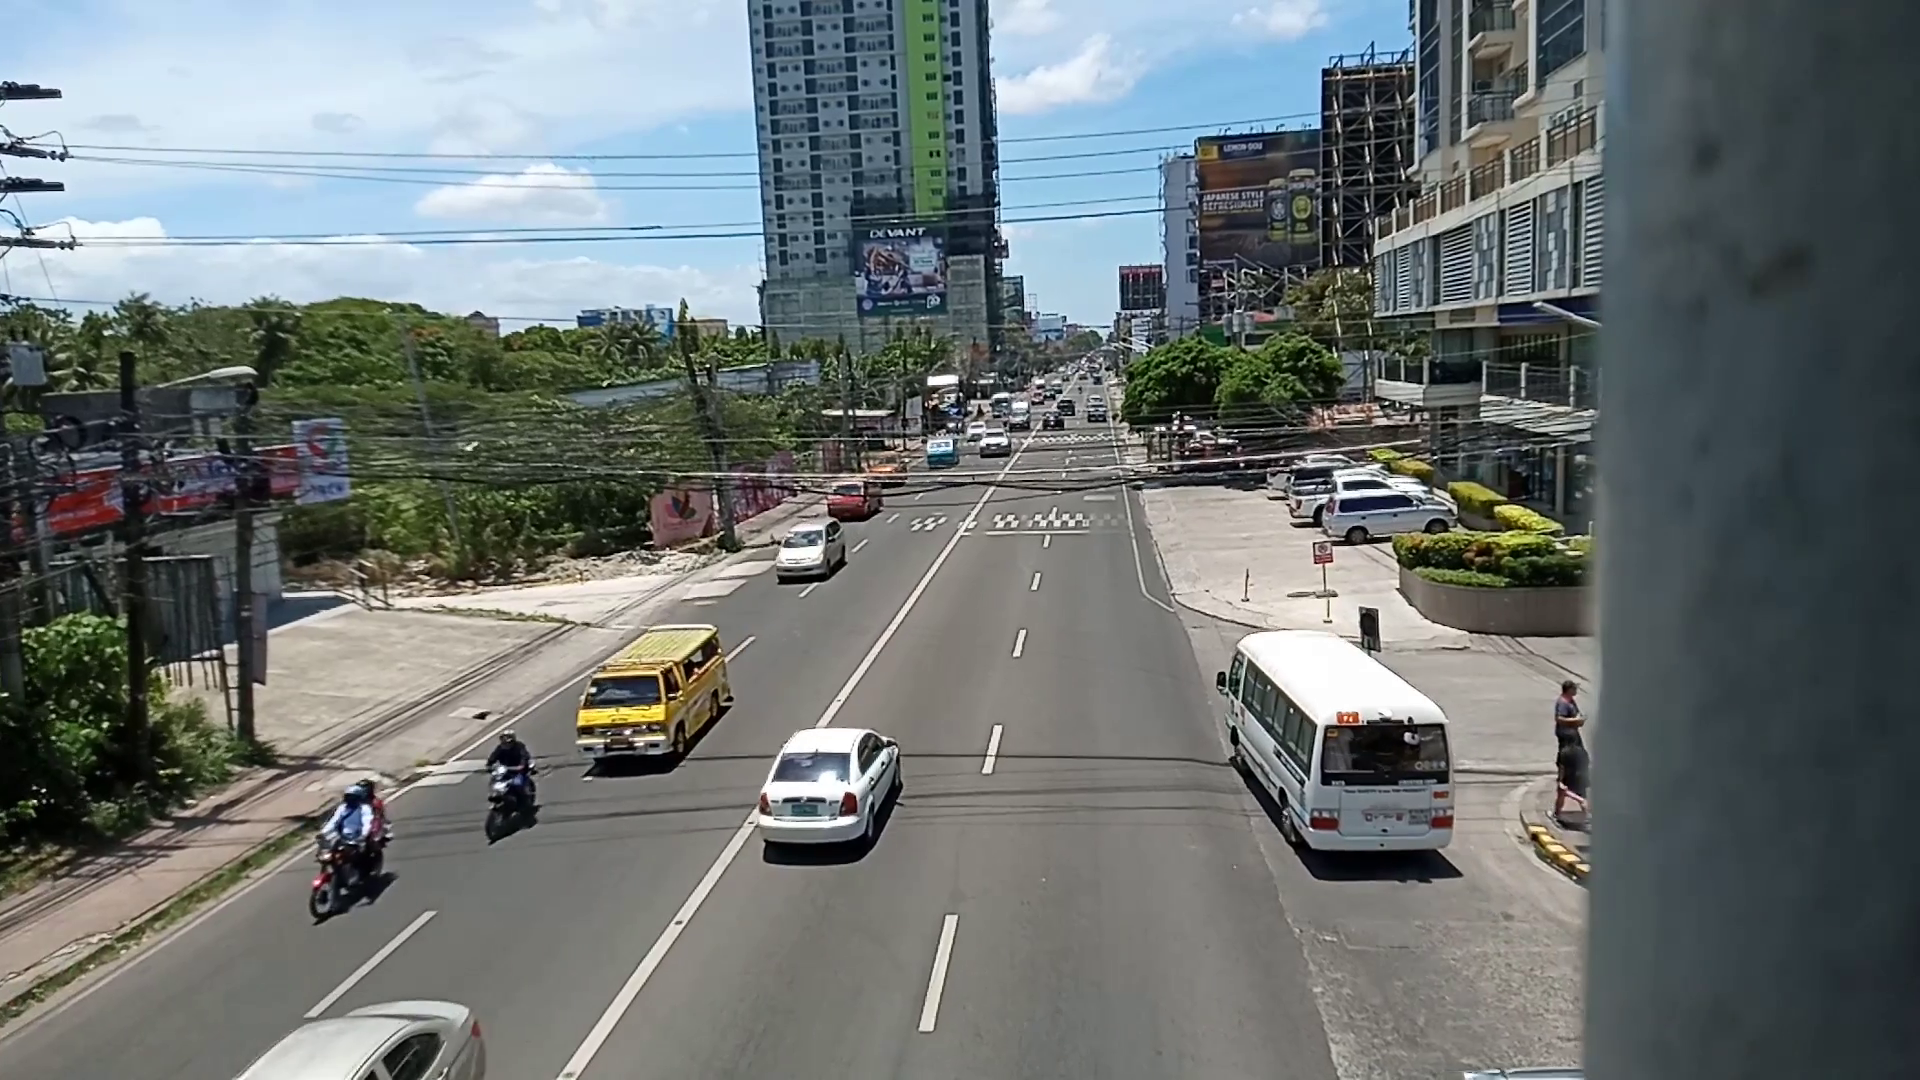
\includegraphics[width=.8\linewidth]{bounding_pics/bacolod_unbound.png}
		\caption{Manual Count: 15 Vehicles}
		
	\end{subfigure}%
	\begin{subfigure}{.5\textwidth}
		\centering
		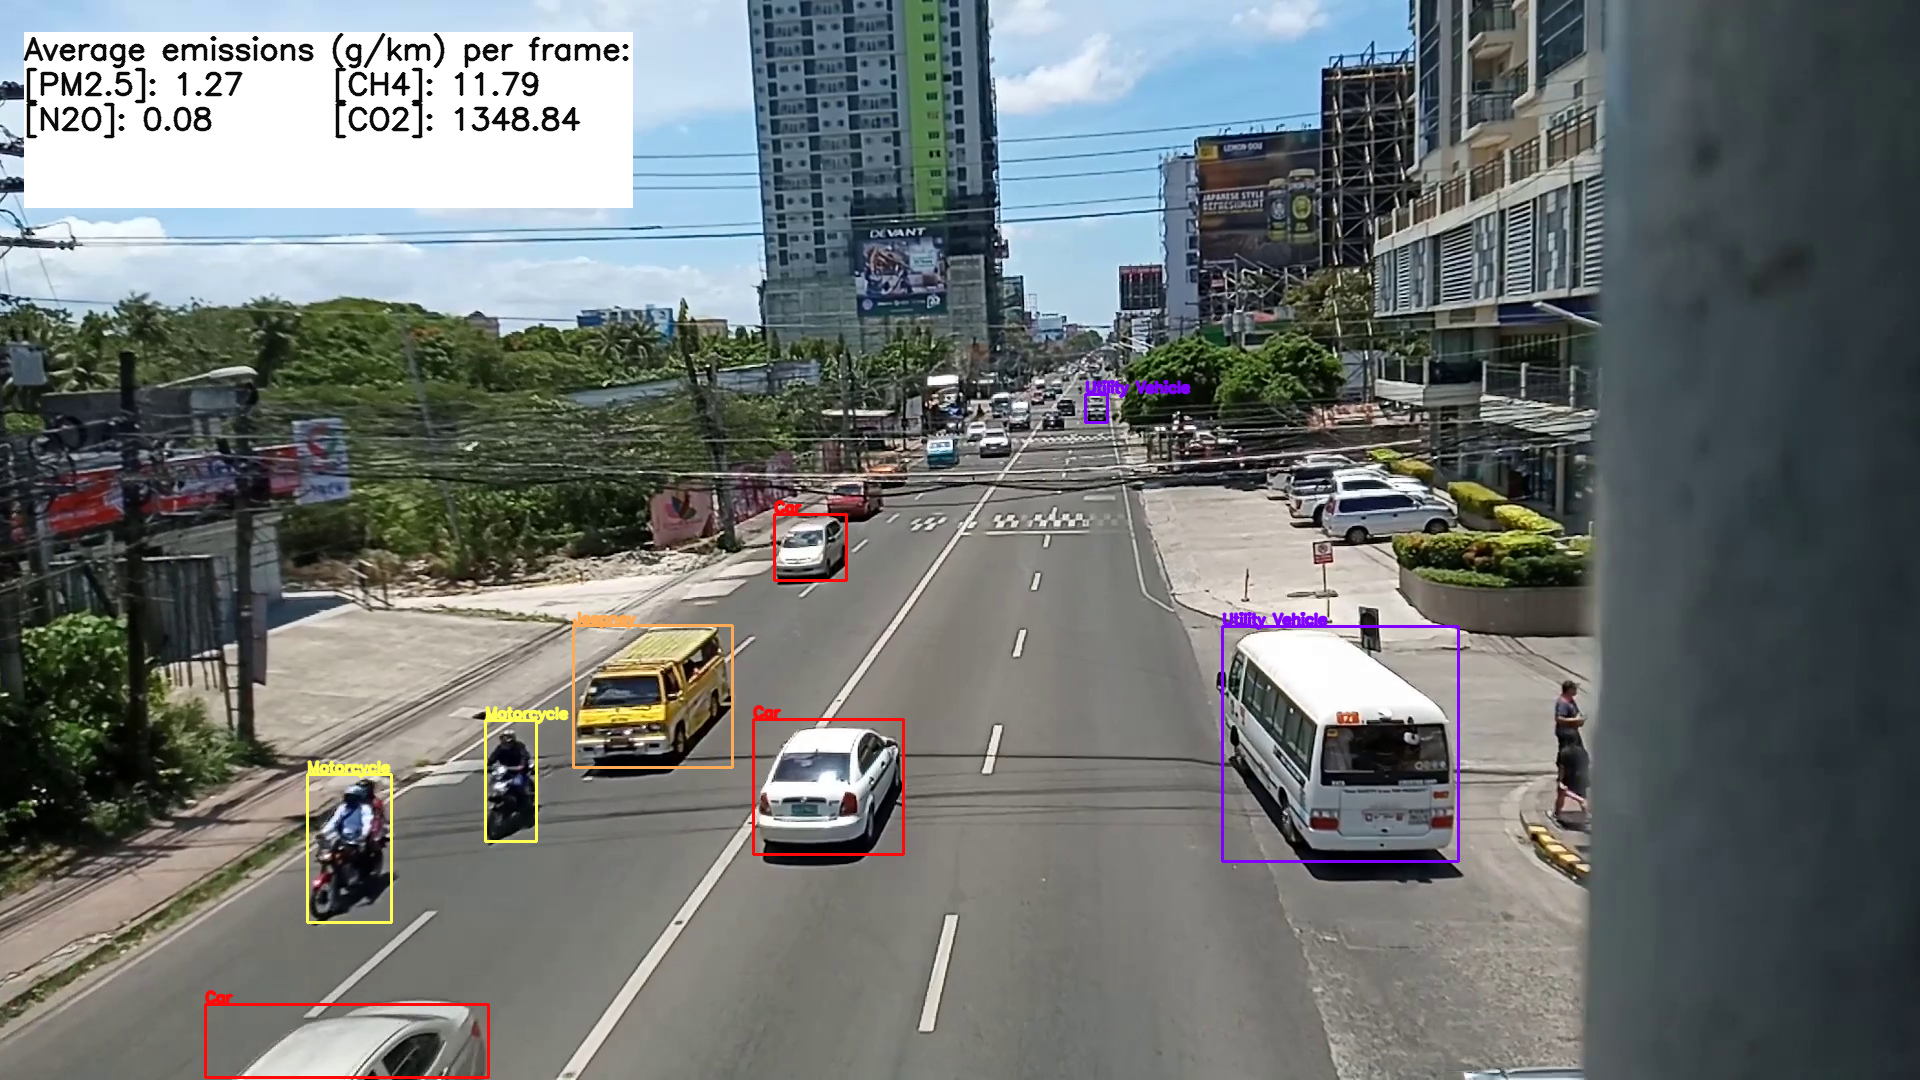
\includegraphics[width=.8\linewidth]{bounding_pics/bacolod_bound.png}
		\caption{Ha.Zee Count: 12 vehicles}
	\end{subfigure}
	\caption{Lacson St. Traffic Video Footage ; Date Taken: 4-7-23, 10:38 AM}
	\label{fig:lacson}
\end{figure}
\FloatBarrier

Using the frames from Figure \ref{fig:lacson} to represent the video footage from Lacson St., Bacolod City; the researchers manually counted 15 total vehicles. The most common vehicle in this frame is the car, with a count of 9. After using the trained model, the system returned a count of 12 vehicles. In this instance, the most common vehicle type detected was also the car, with a count of 5. This being a highway could be the reason why there is a lack of tricycles.

Table \ref{tab:lacson_st} applies the same calculation processes as the previous location. Of the total average of manually-counted vehicles, only 58.42\% were detected by the system. 



\begin{table}[ht]   %t means place on top, replace with b if you want to place at the bottom
	\centering
	\caption{Ratio of Manual vs. Detected average vehicles counted  (Lacson St.)} \vspace{0.25em}
	\begin{tabular}{c|c|c} \hline
		\centering \textbf {Vehicle type} & \textbf{Manual Count Avg.} & \textbf{Ha.Zee Count Avg.} \\ \hline
		Car & 10.45 & 3.18   \\ 
		Jeepney & 2.45 & 1.91  	\\ 
		Motorcycle& 2.27  & 2.09  \\ 
		Tricycle   & 0  & 0.09  \\ 
		UV & 1 & 2.18  \\ 
		Truck & 0 & 0 \\ \hline
		
		\textbf{Total Average} & 16.18 & 9.45  \\ \hline
		
		\textbf{Ratio/Percentage} & \multicolumn{2}{c}{0.5842}  \\ \hline
		
	\end{tabular}
	\label{tab:lacson_st}
\end{table}

\subsubsection{Roxas Ave. (Roxas City, Capiz)
}


\begin{figure}[!htbp]
	\begin{subfigure}{.5\textwidth}
		\centering
		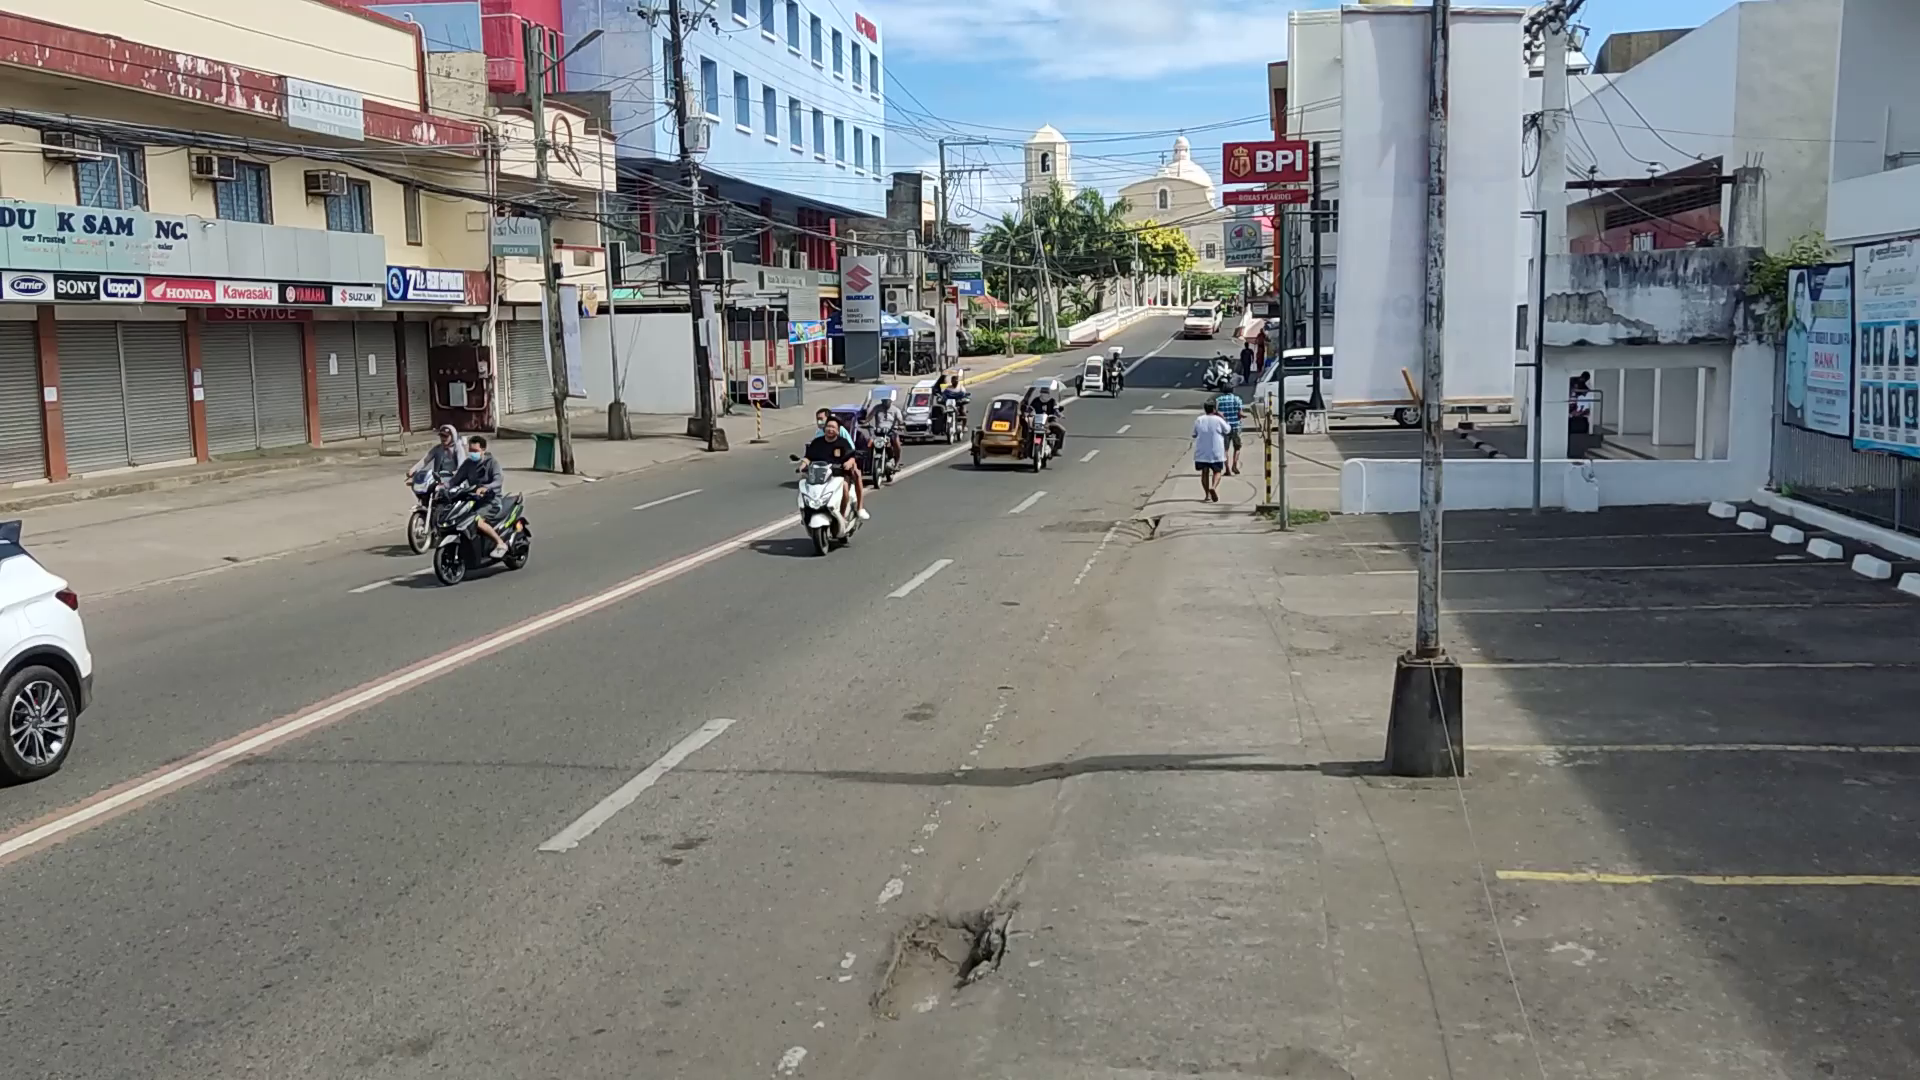
\includegraphics[width=.8\linewidth]{bounding_pics/roxas_unbound.png}
		\caption{Manual Count: 10 Vehicles}
		
	\end{subfigure}%
	\begin{subfigure}{.5\textwidth}
		\centering
		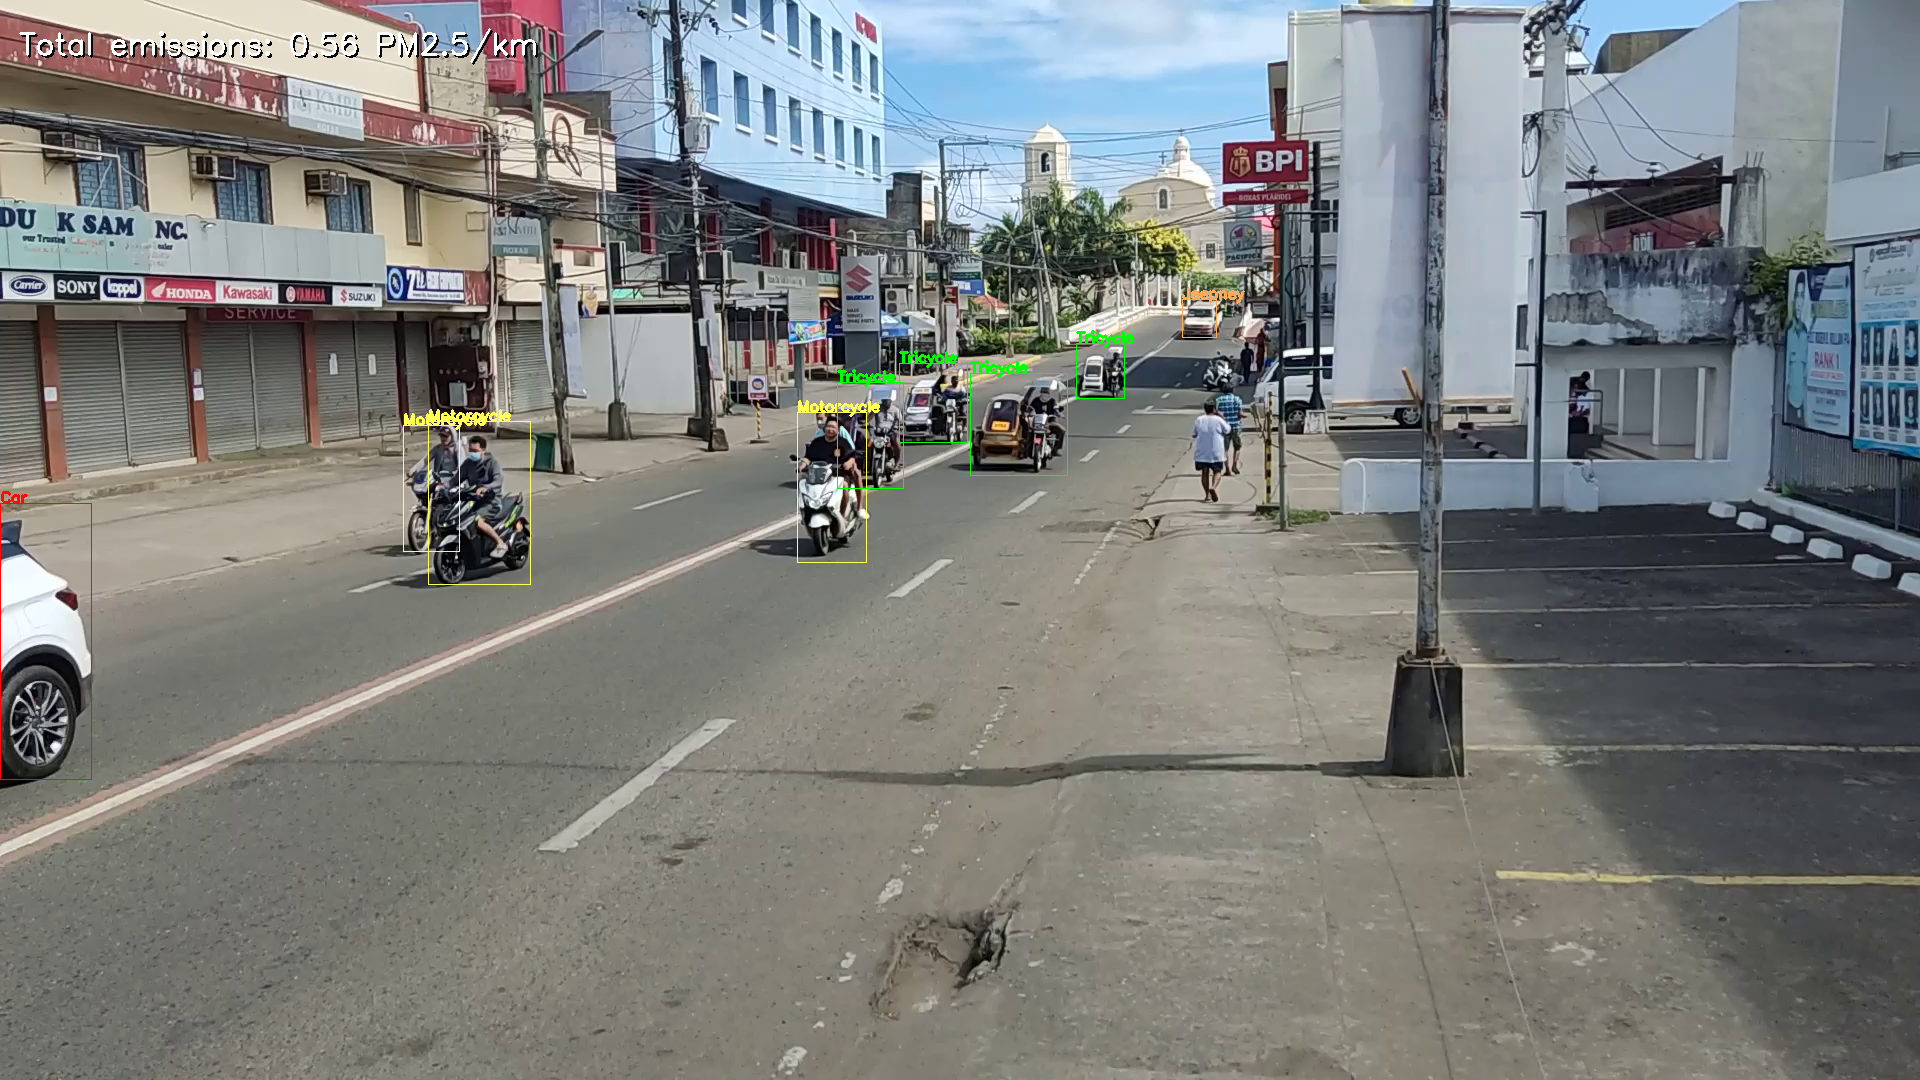
\includegraphics[width=.8\linewidth]{bounding_pics/roxas_bound.png}
		\caption{Ha.Zee Count: 9 vehicles}
	\end{subfigure}
	\caption{Roxas Ave. Traffic Video Footage; Date Taken: 4-8-23, 9:33 AM}
	\label{fig:roxas}
\end{figure}
\FloatBarrier

Using the frames from Figure \ref{fig:roxas} to represent the video footage from  Roxas Ave., Roxas City; the researchers manually counted 10 total vehicles. The most common vehicle in this frame is the tricycle, with a count of 4. After using the trained model, the system returned a count of 9 vehicles. In this instance, the most common vehicle type detected was also the tricycles, with the same count of 4. The high count of Tricycles is due to it being one of the main modes of transportation.

Table \ref{tab:roxas_ave} applies the same calculation processes as the previous location. Of the total average of manually-counted vehicles, only 77.89\% were detected by the system. 



\begin{table}[ht]   %t means place on top, replace with b if you want to place at the bottom
	\centering
	\caption{Ratio of Manual vs. Detected average vehicles counted  (Roxas Ave.)} \vspace{0.25em}
	\begin{tabular}{c|c|c} \hline
		\centering \textbf {Vehicle type} & \textbf{Manual Count Avg.} & \textbf{Ha.Zee Count Avg.} \\ \hline
		Car & 0.90 & 0.54   \\ \hline
		Jeepney & 0.63 & 0.64  	\\ \hline
		Motorcycle& 2.64  & 1.63  \\ \hline
		Tricycle   & 4.45  & 3.72 \\ \hline
		UV & 0 & 0.18  \\ \hline
		Truck & 0 & 0 \\ \hline
		
		\textbf{Total Average} & 8.63 & 6.73 \\ \hline
		\textbf{Ratio/Percentage} & \multicolumn{2}{c}{0.7789}  \\ \hline
		
		
	\end{tabular}
	\label{tab:roxas_ave}
\end{table}

The ratio between of the actual count of the vehicles compared to the amount detected by the system varies between the 5 locations. Roxas Ave., Roxas City’s video footage had the highest percentage of 77.89\%; while Lacson St. in Bacolod City garnered the lowest percentage of 58.42\%. A factor on why Roxas Ave.’s average of vehicles detected is much closer to the average of the actual vehicles manually counted could be due to the fewer vehicles present and their distance from one another. Said distances could have also been the reason why Diversion Road’s detected cars are significantly lesser than the counted vehicles, as some cars were obstructed by other vehicles and are sometimes counted as a singular vehicle. Another factor that affected the percentages could have been the quality of the video footage used in the study. All the footages shown in the figures were taken from the smartphones of the researchers and rendered some vehicles pixelated, which led to some vehicles being indistinguishable to the system. 



\begin{table}[ht]   %t means place on top, replace with b if you want to place at the bottom
	\centering
	\caption{Average Percentage of Ha.Zee-detected Vehicles.} \vspace{0.25em}
	\begin{tabular}{c|c} \hline
		\centering \textbf {Location} & \textbf {Ratio/Percentages} \\ \hline
		Valeria St. & 0.6498 \\
		De Leon St. & 0.7328 	\\ 
		Diversion Road& 0.7160   \\ 
		Lacson St.   & 0.5842  \\ 
		Roxas Ave.  & 0.7789 \\ \hline
		
		\textbf{Total Average} & 0.6923 \\ \hline
		
	\end{tabular}
	\label{tab:avg_perc}
\end{table}


Across the 5 locations, the system is averaged to detect 69.23\% of the vehicles on a given video footage. This is a reasonably acceptable rate and could be improved upon if more data on different vehicles of varying image qualities were to be added to the training of the system.

\section{Pollutant Estimation Comparison and Interpretation}

\subsection{Average Pollutant Per Location}
The pollutant estimation displayed on the upper left of the Ha.Zee system were calculated at an interval of 1 frame per second. The displayed data is calculated using the equation given in section 3.3.1. Due to the limitations of the study, the pollutant values displayed pertains to the emission from vehicles only. Factors such as smoke from industrial buildings, fireplaces, etc. are not accounted for in the equation. Table \ref{tab:avg_emission} compared the averages of the estimated $PM_{2.5}$, \ch{N2O}, \ch{CH4}, and \ch{CO2} emissions per of the 5 locations via finding the mean across every frame.

\begin{table}[ht]   %t means place on top, replace with b if you want to place at the bottom
	\centering
	\caption{Average pollutant estimation across different locations} \vspace{0.25em}
	\begin{tabular}{c|c|c|c|c} \hline
		\centering \textbf {Location}  & $PM_{2.5}$ &\ch{CH4} & \ch{N2O} & \ch{CO2} \\ \hline
		Valeria St. & 6.807272727 & 14.74272727 & 0.3009090909 & 5947.653636\\
		De Leon St. & 2.422 & 23.79733333 & 0.1126666667 & 2238.534	\\ 
		Diversion Road& 7.339090909 & 26.13 & 0.54 & 8403.652727 \\ 
		Lacson St.   & 1.272727273 & 8.218181818 & 0.07818181818 & 1308.494545\\ 
		Roxas Ave.  & 0.738125 & 19.75875 & 0.04 & 839.34875 \\ \hline

		
	\end{tabular}
	\label{tab:avg_emission}
\end{table}


As seen on the table, the highest average pollutant estimation among the different locations is Diversion Road. Meanwhile, Roxas ave. has the lowest average estimation. The reason why Diversion road reached those values is explained by its status as highway road, wherein it can accommodate a large number of vehicles. Meanwhile, Roxas ave. is a two-lane road, accommodating less vehicles than the other roads in the study. Valeria St., though being a one-way road and smaller than the road of De Leon St., has the second highest average pollutant values. This is due to the amount of jeepneys present in the footage having higher emission values, increasing the average while having lesser vehicles present.

Aside from road size, another factor to the varying pollutant estimations would be the traffic density based on the time the footage was taken. Instances such as rush hours could potentially impact a location's pollutant estimation.

\subsection{Pollutant Contribution per Vehicle}

To assess the vehicle type that contributes the most to each pollutant, we calculated the average vehicle count per frame and multiply it by the available emission value of each pollutant from each vehicle. The resulting calculations are presented in Table \ref{tab:avg_pollutant} .This allows for determining the contributions of different vehicle types to the overall pollutant levels, allowing for a better understanding of the environmental impact of each vehicle type.

\begin{table}[ht]   %t means place on top, replace with b if you want to place at the bottom
	\centering
	\caption{Average pollutant contribution of each type of vehicle per frame} \vspace{0.25em}
	\begin{tabular}{p{2in}|c|c|c|c} \hline
		\centering \textbf{Vehicle Type} & $PM_{2.5}$ &\ch{CH4} & \ch{N2O} & \ch{CO2} \\ \hline
		Tricycle   & 0.10713125   & 7.79770625 & 0.004003125 & 127.4798969 \\
		Motorcycle& 0.063  & 4.316625  & 0.0028125 & 112.6843125 \\ 
		Jeepney &2.77790625&0.773390625 &0.1036875	& 2194.308047\\ 
		Car & 0.1598796875 & 5.359225 & 0.0716203125 & 795.0274281\\ 
		Utility Vehicle & 0.283765625 & 0.702071875 & 0.0125015625 & 183.3639891\\ 
		Light Truck & 0.0117484375 & 0.0057 & 0.000353125& 13.15758125\\ \hline
		
	\end{tabular}
	\label{tab:avg_pollutant}
\end{table}

It is essential to emphasize that the presented values reflect the collected data and may not represent the overall contributions of each vehicle type to pollutants. However, based on the data analysis, certain trends can be observed.

For pollutants $PM_{2.5}$, \ch{N2O}, and \ch{CO2}; the "Jeepney" class demonstrates the highest contribution. This high contribution can be attributed to the "Jeepney" class having the highest emission levels per vehicle for $PM_{2.5}$ and \ch{N2O}. In the case of \ch{CO2}, while the "Jeepney" class ranks second in terms of emission levels per vehicle, the scarcity of "Truck" objects in the captured data resulted in the "Jeepney" class having a higher overall contribution to \ch{CO2} emissions.

The "Tricycle" class exhibits the highest contribution to CH4 emissions, which can be attributed to its higher CH4 emission levels per vehicle compared to other classes.
Conversely, the "Truck" class demonstrates the least contribution to every pollutant. This is primarily due to the scarcity of "Truck" objects in the captured data, resulting in fewer instances of emission and consequently lower overall contribution to the pollutant levels analyzed.

It is important to interpret these findings within the context of the specific dataset used, understanding that they may not generalize to the broader population of vehicles and pollutant contributions.

